% Created 2022-06-10 Fri 17:14
% Intended LaTeX compiler: pdflatex
\documentclass[11pt]{article}
\usepackage[utf8]{inputenc}
\usepackage[T1]{fontenc}
\usepackage{graphicx}
\usepackage{grffile}
\usepackage{longtable}
\usepackage{wrapfig}
\usepackage{rotating}
\usepackage[normalem]{ulem}
\usepackage{amsmath}
\usepackage{textcomp}
\usepackage{amssymb}
\usepackage{capt-of}
\usepackage{hyperref}
\author{zhou yang}
\date{\today}
\title{}
\hypersetup{
 pdfauthor={zhou yang},
 pdftitle={},
 pdfkeywords={},
 pdfsubject={},
 pdfcreator={Emacs 27.1 (Org mode 9.4.4)}, 
 pdflang={English}}
\begin{document}

\tableofcontents

\section{numpy learning}
\label{sec:org7e823a9}

\subsection{axis=i}
\label{sec:org31f4c9c}
\subsubsection{apply operations on each elements of i-th index (element in the (i+1)-th square bracket) of the shape}
\label{sec:org6b7a434}
\subsubsection{example: 2d:}
\label{sec:org1df6e64}
\subsubsection{axis=0, vertical, axis = 1, horizontally, axis=3, can be viewed as operate horizontally on the element of a[0,\ldots{}]}
\label{sec:org0eca6a0}
\subsection{basics}
\label{sec:orgc2f0db6}
\subsubsection{ndarray: with an alias array, and axis means dim}
\label{sec:orgd0e81fb}
\subsubsection{Attributes}
\label{sec:org7b7e9c1}
\begin{enumerate}
\item ndarray.ndim:=len(ndarray.shape) =rank, which no. of dims (axis)
\label{sec:org3567539}
\item ndarray.shape: (n, m): a tuple of integer, with each element denoting the no. of element in the corresponding dim
\label{sec:orgc2504de}
\item ndarray.size: = total no. of elements = ndarray.shape[0]* ndarray.shape[1]
\label{sec:org8123884}
\item ndarray.dtype: the type of elements in the ndarray
\label{sec:org9a0e9d5}
\item ndarray.itemsize: the byte size for each element= bits/8
\label{sec:orge038762}
\item ndarray.data: the data in cache (memory) of the array
\label{sec:org9500467}
\end{enumerate}
\subsubsection{example}
\label{sec:org5c6dd75}
\subsubsection{method}
\label{sec:org471267e}
\begin{enumerate}
\item reshape(): won't change the original ndarray
\label{sec:orgd9a9226}
\item flatten(): return a new flatten to 1-d array
\label{sec:orgbf30283}
\item astype(): return a new array with the specified data type
\label{sec:org8b0186c}
\item sum(): sum up along axis
\label{sec:orga22dc29}
\item cumsum():
\label{sec:org515bb4d}
\item max():
\label{sec:org3a48d27}
\item min():
\label{sec:orgeff4bd2}
\item mean():
\label{sec:orgde48305}
\end{enumerate}
\subsubsection{how to create ndarray}
\label{sec:org79b7f33}
\begin{enumerate}
\item np.array( a python list, or tuple, or list of tuple): the dtype is inferred from data
\label{sec:org3aedcad}
\begin{enumerate}
\item np.array([\ldots{}], dtype=complex): the dtype can be specified
\label{sec:org25b896d}
\end{enumerate}
\item np.asarray(arr\textsubscript{like}, dtype=None, order=None):
\label{sec:org777774e}
\item np.fromiter(iterable, dtype, count=-1):build array from iterable
\label{sec:org7abcdfe}
\begin{enumerate}
\item The number of items to read from \textbf{iterable}.  The default is -1,which means all data is read.
\label{sec:org0996471}
\end{enumerate}
\item np.logspace(start, stop, num=50, base=10.0, dtype=None):
\label{sec:org228a2a9}
\begin{enumerate}
\item In linear space, the sequence starts at ``base \textbf{* start``(`base` to the power of `start`) and ends with ``base *} stop``
\label{sec:orgbb7f871}
\item 
\label{sec:org78abe58}
\end{enumerate}
\item np.full(shape, fill\textsubscript{value}): return an array with the specified shape and value
\label{sec:org23139ee}
\item np.random.random(shape)
\label{sec:org88af4cd}
\item np.eye(n\textsubscript{dims})
\label{sec:org17d308d}
\item np.diag(list\textsubscript{of}\textsubscript{values}): return a diagonal array with the specified diagonal values
\label{sec:orgd9819ad}
\item np.zeros(shape: a tuple or an int for 1d array): the default dtype is 'float64'
\label{sec:orgb99c6b8}
\begin{enumerate}
\item np.zeros\textsubscript{like}()
\label{sec:org7660198}
\end{enumerate}
\item np.empty(shape: a 2d tuple): its values are randomly init, with default dtype is float64
\label{sec:org8801866}
\begin{enumerate}
\item np.empty\textsubscript{like}()
\label{sec:org30ca2ab}
\end{enumerate}
\item np.arange(start, end, step): return an array. When used with float parameters, cannot control the no. of elements created, solution: linspace
\label{sec:orga29e139}
\item np.linspace(start, end, no of elements):
\label{sec:orge1ea7cc}
\item np.ones()
\label{sec:orgcc3b376}
\begin{enumerate}
\item np.ones\textsubscript{like}()
\label{sec:org04a5a39}
\end{enumerate}
\item np.fromfunction(function, shape, dtype):
\label{sec:org2aede6b}
\begin{enumerate}
\item (N,) tuple of ints Shape of the output array, which also determines the shape of the coordinate arrays passed to `function`.
\label{sec:org2c90c23}
\item function(index\textsubscript{1}): for 1d or function(index\textsubscript{1}, index\textsubscript{2}) for 2d, where index\textsubscript{i} in np.arange(shape[i])
\label{sec:org74c1c42}
\end{enumerate}
\end{enumerate}
\subsubsection{create bool array}
\label{sec:orgc7e747c}
\begin{enumerate}
\item b = np.array([1,0, 3,0], dtype=bool)
\label{sec:orga37f09c}
\end{enumerate}
\subsubsection{print the whole array}
\label{sec:orgb11d58c}
\begin{enumerate}
\item np.set\textsubscript{printoptions}(threshold=sys.maxsize)       \# sys module should be imported
\label{sec:orgca605b3}
\end{enumerate}
\subsection{index}
\label{sec:orgeff23e5}
\subsubsection{index of an array can be any list, array or tuple}
\label{sec:org1edd092}
\begin{enumerate}
\item a[1:4] == a[ [0,1,2,3] ]
\label{sec:orgc5a8583}
\item a[array([1,2])] is legal
\label{sec:org0b10a9c}
\end{enumerate}
\subsection{basic operations}
\label{sec:org25ba90e}
\subsubsection{the math operations on an array will be applied on each element}
\label{sec:org99b50ac}
\begin{verbatim}
a = np.array( [20,30,40,50] )
b = np.arange( 4 )
c = a-b # array([20, 29, 38, 47])
b**2 # array([0, 1, 4, 9])
a<35 # array([ True, True, False, False])
\end{verbatim}
\subsubsection{'$\backslash$*': element-wised multiplication}
\label{sec:orgd7aeffa}
\subsubsection{matrix multiplication: @ or 'dot' function (python>=3.5) A*B, A.dot(B)}
\label{sec:org7bb8099}
\subsubsection{some operations can modify array in place: such as '+=', `*=`}
\label{sec:org7da98d9}
\begin{enumerate}
\item a += b: it requires that b can be automatically converted to the type of a, o.w., error
\label{sec:orgfd3da96}
\item a(int) += b(float): error
\label{sec:orge22ef58}
\item the result of operations involving different types of array:
\label{sec:org72b270f}
\begin{enumerate}
\item cast to the higher precision representation
\label{sec:orga3a3ab7}
\end{enumerate}
\end{enumerate}
\subsubsection{unary-operation: one element}
\label{sec:org46ed59f}
\begin{enumerate}
\item a.sum():
\label{sec:orgf2de8b8}
\item a.min():
\label{sec:org27ce998}
\item a.max():
\label{sec:orgda1828f}
\item can be applied on given axis
\label{sec:orgc8bea1a}
\begin{enumerate}
\item b.sum(axis=None) \# sum of each column, axis default is None, denoting sum all
\label{sec:orgc900a5f}
\item b.min(axis=0) \# min of each row, default is None, axis default is None
\label{sec:orgf6b376c}
\item b.cumsum(axis=1) \# cumulative sum along each row, axis default is None
\label{sec:orgdd59c61}
\end{enumerate}
\end{enumerate}
\subsubsection{ufunc: universal function}
\label{sec:orgc52b03a}
\begin{enumerate}
\item operates in an element-by-element fashion, supporting array broadcasting, type casting, and several other standard features.
\label{sec:orgb5c9016}
\item example, sin, cos, exp, sqrt, add
\label{sec:org3b69a4c}
\end{enumerate}
\subsubsection{slicing}
\label{sec:org7858e6f}
\begin{enumerate}
\item a[ : :-1]: revert the array
\label{sec:org3668499}
\item the slicing can be performed on each axis: a[1:3, 2:3]
\label{sec:org4b1bc88}
\item when slicing is performed on a no axis that less than rank, the slicing on the missing axis is set to be all along the axis, that is ':'
\label{sec:org0738e16}
\begin{enumerate}
\item b.shape-> (2, 3), b[-1]-> =b[-1, :] \# the last row
\label{sec:org7fb1cb5}
\item b[i] = b[i,:] = b[i,\ldots{}]
\label{sec:org727aaaf}
\item '\ldots{}': denote the rest of the index, take for example x, x has rank five, len(x.shape) ->5
\label{sec:org7a312a5}
\item x[1,2,\ldots{}] = x[1,2,:,:,:],
\label{sec:org76a0fbf}
\item x[\ldots{},3] = x[:,:,:,:,3]
\label{sec:org2004d96}
\item x[4,\ldots{},5,:] = x[4,:,:,5,:]
\label{sec:orgadae4ee}
\end{enumerate}
\item when iterate over a ndarray, it is on the first dim
\label{sec:orgfcc5a8c}
\begin{enumerate}
\item for row in b: print(row)
\label{sec:org8b347a2}
\end{enumerate}
\item to iterate over every item, we can use the 'flat' attribute, which is the generator of all the elements
\label{sec:org2adf4c2}
\begin{enumerate}
\item a.flat: attribute, return a flat iterator over an array, return type: <class 'numpy.flatiter'>
\label{sec:org3879590}
\item a.flatten():Returns a flattened copy of an array.
\label{sec:orge6fc069}
\item for element in b.flat: print(element)
\label{sec:orge131d8f}
\end{enumerate}
\end{enumerate}
\subsubsection{operation on the shape}
\label{sec:org7cc0e44}
\begin{enumerate}
\item the following operations can change the shape of an array, and return the modified array, but the original one is unchanged
\label{sec:org8f263e9}
\item a.shape = x,y \# can also
\label{sec:org51a6426}
\item a.ravel()  \# returns the array, flattened
\label{sec:orge5f1e30}
\item a.reshape(6,2) \# return the array with a modified shape
\label{sec:org3686c00}
\begin{enumerate}
\item a.reshanp.vstack()np.hstack()pe(shape=ints or a tuple of int)
\label{sec:org0d32535}
\item if the snp.vstack()np.hstack()ize =-1, the dimension will be inferred automatically
\label{sec:orgaf8b91d}
\end{enumerate}
\item a.resize(new\textsubscript{shape}): change shape and size of array in-place
\label{sec:org8a09187}
\item a.T \# return the transposed array
\label{sec:orgb4b286c}
\item ndarray.resize(): will change the original array
\label{sec:org1b7cc11}
\end{enumerate}
\subsubsection{array stacking and concatenating}
\label{sec:org233ae96}
\begin{enumerate}
\item np.vstack(): stack vertically
\label{sec:org2f64911}
\item np.hstack(): stack horizontally
\label{sec:orgc1ca333}
\begin{enumerate}
\item np.floor(): return the floor value element-wised
\label{sec:orgb29b2ac}
\end{enumerate}
\item np.column\textsubscript{stack}():
\label{sec:org2e7c798}
\begin{enumerate}
\item Stack 1-D arrays as columns into a 2-D array.
\label{sec:orgf1e43e1}
\item 2-D arrays are stacked as-is, just like with `np.hstack()`
\label{sec:org5f6a8e0}
\item a = np.array([4.,2.]), b = np.array([3.,8.]), np.column\textsubscript{stack}((a,b)) -> array([[ 4., 3.], [ 2., 8.]])
\label{sec:orga25bb1c}
\item np.hstack((a,b)) -> array([ 4., 2., 3., 8.])
\label{sec:org7de9d9e}
\item a[:,newaxis] \# this allows to have a 2D columns vector -> array([[ 4.], [ 2.]])
\label{sec:orgc0a2241}
\item np.column\textsubscript{stack}((a[:,newaxis],b[:,newaxis])) = np.hstack((a[:,newaxis],b[:,newaxis]))
\label{sec:org8e4493b}
\end{enumerate}
\item np.row\textsubscript{stack}() = np.vstack() for any shape of input.
\label{sec:orge12223b}
\end{enumerate}
\subsubsection{np.r\_ and np.c\_}
\label{sec:orgb70ba27}
\begin{enumerate}
\item np.r\_[1:4, 0, 4]->array([1, 2, 3, 0, 4]): create array along an axis
\label{sec:org6bdef5f}
\item when used with array parameters, the r\_ = vstack, c\_ = hstack, and allows to specify the axis to concatenate
\label{sec:org3077342}
\end{enumerate}
\subsubsection{splitting an array}
\label{sec:org3379b04}
\begin{enumerate}
\item np.hsplit(a, 3) \# split a into 3 array
\label{sec:org9de2dbf}
\item np.hsplit(a (3, 4)) \# split a after the third and the fourth column
\label{sec:orgf28363f}
\item np.vsplit(): split vertically
\label{sec:org02bb859}
\item np.array\textsubscript{split}(): split along the specified axis
\label{sec:orgef78aec}
\end{enumerate}
\subsubsection{copy and view}
\label{sec:org72e1f73}
\begin{enumerate}
\item making alias of a array won't copy the array
\label{sec:org008d50e}
\begin{enumerate}
\item a = np.arange(10), b = a, \#b is an alias of a
\label{sec:org991dabb}
\end{enumerate}
\item passing an changeable object to a function won't copy the object
\label{sec:orgbd0ffac}
\begin{enumerate}
\item def (x):print(id(x)), f(a):  a and x point to the same array
\label{sec:org59ead7e}
\end{enumerate}
\item view and shallow copy
\label{sec:org1057bd0}
\begin{enumerate}
\item different array can share the same data.
\label{sec:org8c9ffad}
\item view(): New view of array with the same data.
\label{sec:org57e2d01}
\begin{enumerate}
\item c = a.view(), \# c is a view of the data owned by a
\label{sec:org29f6046}
\item c.flags.owndata -> false
\label{sec:org9addfa6}
\item change the shape of c won't affect the the shape of a
\label{sec:orgc8e025c}
\item but change the value of c will change the value of a
\label{sec:orgc2beec6}
\end{enumerate}
\item slicing will return a view of the original data, which is an alias instead of a copy.
\label{sec:orgb151429}
\begin{enumerate}
\item s = a[:, 1:3], \# return a view of the data owned by a
\label{sec:org943bb15}
\item s[:] = 10, vs s=10, there are different, the former change the data of a
\label{sec:org7f703f2}
\end{enumerate}
\end{enumerate}
\item deep copy: copy data and create new array
\label{sec:org94b1c06}
\begin{enumerate}
\item if the original array is not needed, should use the copy() after slicing
\label{sec:org80c2c8f}
\item b = a[:100].copy, del a, \# assume a is a large intermediary result
\label{sec:org309fbc7}
\item if b = a[:100], when deleting a, the a will persist in the memory
\label{sec:org1907af5}
\end{enumerate}
\end{enumerate}
\subsection{Method}
\label{sec:org74d7bb1}
\subsubsection{frequently used method}
\label{sec:orgd923149}
\begin{enumerate}
\item Array Creation - arange, array, copy, empty, empty\textsubscript{like}, eye, fromfile, fromfunction, identity, linspace, logspace, mgrid, ogrid, ones, ones\textsubscript{like}, zeros, zeros\textsubscript{like}
\label{sec:orgbca94fa}
\item Conversions - ndarray.astype, atleast\textsubscript{1d}, atleast\textsubscript{2d}, atleast\textsubscript{3d}, mat
\label{sec:orgec3a860}
\item Manipulations - array\textsubscript{split}, column\textsubscript{stack}, concatenate, diagonal, dsplit, dstack, hsplit, hstack, ndarray.item, newaxis, ravel, repeat, reshape, resize, squeeze, swapaxes, take, transpose, vsplit, vstack
\label{sec:org9963674}
\item Questions - all, any, nonzero, where,np.vstack()np.hstack()
\label{sec:org8ae5aeb}
\item Ordering - argmax, argmin, argsort, max, min, ptp, searchsorted, sort
\label{sec:orgb334bf7}
\item Operations - choose, compress, cumprod, cumsum, inner, ndarray.fill, imag, prod, put, putmask, real, sum
\label{sec:org6c94ef5}
\item Basic Statistics - cov, mean, std, var
\label{sec:orgb88628e}
\item Basic Linear Algebra - cross, dot, outer, linalg.svd, vdot
\label{sec:org05c2e65}
\end{enumerate}
\subsubsection{broadcasting}
\label{sec:org0d11d3c}
\begin{enumerate}
\item ruels: When operating on two arrays, NumPy compares their shapes element-wise. It starts with the trailing (i.e. rightmost) dimensions and works its way left. Two dimensions are compatible when they are equal, or one of them is 1
\label{sec:org1a0cbd8}
\begin{enumerate}
\item I.if all the input arrays have different shape, then "1" is used to fill the smallest array such that they have the same shape
\label{sec:org74fb1dd}
\end{enumerate}
\item example: x = np.arange(4), xx = x.reshape(4,1), y = np.ones(5), z = np.ones((3,4)), x and xx can be broadcast, but x and y are not
\label{sec:orgc1951da}
\end{enumerate}
\subsection{more slicingnp.vstack()np.hstack()}
\label{sec:orgaf8e078}
\begin{verbatim}
>>> a = np.arange(12)**2                       # the first 12 square numbers
>>> i = np.array( [ 1,1,3,8,5 ] )              # an array of indices
>>> a[i]                                       # the elements of a at the positions i
array([ 1,  1,  9, 64, 25])
>>>
>>> j = np.array( [ [ 3, 4], [ 9, 7 ] ] )      # a bidimensional array of indices
>>> a[j]                                       # the same shape as j
array([[ 9, 16],
       [81, 49]])
# when the rank(a)>1, a single index of array indicates the first dim of a.
>>> palette = np.array( [ [0,0,0],                # black
...                       [255,0,0],              # red
...                       [0,255,0],              # green
...                       [0,0,255],              # blue
...                       [255,255,255] ] )       # white
>>> image = np.array( [ [ 0, 1, 2, 0 ],           # each value corresponds to a color in the palette
...                     [ 0, 3, 4, 0 ]  ] )
>>> palette[image]                            # the (2,4,3) color image
array([[[  0,   0,   0],
        [255,   0,   0],
        [  0, 255,   0],
        [  0,   0,   0]],
       [[  0,   0,   0],
        [  0,   0, 255],
        [255, 255, 255],
        [  0,   0,   0]]])

# we can provide multiple index arrays, and every array should have the same shape
>>> a = np.arange(12).reshape(3,4)
>>> anp.vstack()np.hstack()
array([[ 0,  1,  2,  3],
       [ 4,  5,  6,  7],
       [ 8,  9, 10, 11]])
>>> i = np.array( [ [0,1],                        # indices for the first dim of a
...                 [1,2] ] )
>>> j = np.array( [ [2,1],                        # indices for the second dim
...                 [3,3] ] )
>>>
>>> a[i,j]                                     # i and j must have equal shape
array([[ 2,  5],
       [ 7, 11]])
>>>
>>> a[i,2]
array([[ 2,  6],
       [ 6, 10]])
>>>
>>> a[:,j]                                     # i.e., a[ : , j]
array([[[ 2,  1],
        [ 3,  3]],
       [[ 6,  5],
        [ 7,  7]],
       [[10,  9],
        [11, 11]]])
# equivalently we can have
>>> l = [i,j]
>>> a[l]                                       # equivalent to a[i,j]
array([[ 2,  5],
       [ 7, 11]])


# index can be used to assign new value
>>> a = np.arange(5)
>>> a
array([0, 1, 2, 3, 4])
>>> a[[1,3,4]] = 0
>>> a
array([0, 0, 2, 0, 0])

# when a index is used to assign value multiple times, it keeps the last oen
>>> a = np.arange(5)
>>> a[[0,0,2]]=[1,2,3]
>>> a
array([2, 1, 3, 3, 4])

# when using with '+=', the result may be unexpected
>>> a = np.arange(5)
>>> a[[0,0,2]]+=1
>>> a
array([1, 1, 3, 3, 4]) # though 0 appears twice, but it increases by 1

\end{verbatim}
\subsection{bool slicing}
\label{sec:org6ba93e0}
\subsubsection{I.use a bool array that has the same shape with the original array}
\label{sec:org9b2dca4}
\subsubsection{Slicing on the first dim}
\label{sec:orgcca6cba}




\begin{verbatim}
>>> a = np.arange(12).reshape(3,4)
>>> b = a > 4np.vstack()np.hstack()
>>> b                                          # b is a boolean with a's shape
array([[False, False, False, False],
       [False,  True,  True,  True],
       [ True,  True,  True,  True]])
>>> a[b]                                       # 1d array with the selected elements
array([ 5,  6,  7,  8,  9, 10, 11])

# this one is frequently used in assigning values
>>> a[b] = 0                                   # All elements of 'a' higher than 4 become 0
>>> a
array([[0, 1, 2, 3],
       [4, 0, 0, 0],
       [0, 0, 0, 0]])
\end{verbatim}
\subsubsection{For each dim, we can have a boolean filter, but the length of the filter must match the length of the targeted dim}
\label{sec:org0bf939e}
\#+begin\textsubscript{src} python
>>> a = np.arange(12).reshape(3,4)
>>> b1 = np.array([False,Trunp.vstack()np.hstack()e,True])             \# first dim selection
>>> b2 = np.array([True,False,True,False])       \# second dim selection
a[b1,:]                                   \# selecting rows
array([[ 4,  5,  6,  7],
       [ 8,  9, 10, 11]])
a[b1,b2]                                  \# a weird thing to do
array([ 4, 10]) 
\begin{verbatim}
stack two 1d array to have a 2d array: stack two 1d array to have a 2d array: stack two 1d array to have a 2d array: stack two 1d array to have a 2d array: stack two 1d array to have a 2d array: stack two 1d array to have a 2d array: stack two 1d array to have a 2d array#+end_src
\end{verbatim}
\subsection{ix\textsubscript{()} function}
\label{sec:org3cfb482}
\subsubsection{ix\textsubscript{()} can be used to combine different vectors in a way to generate n-tuple}
\label{sec:orgf5ccafa}
\begin{enumerate}
\item example: for vector a, b and c, we show all the combinations of them in a+b*c
\label{sec:orgfc8ed59}
\begin{verbatim}
>>> a = np.array([2,3,4,5])
>>> b = np.array([8,5,4])
>>> c = np.array([5,4,6,8,3])
>>> ax,bx,cx = np.ix_(a,b,c) # ax.shape= (4, 1, 1), bx.shape= (1, 3, 1), cx.shape= (1, 1, 5)
>>> result = ax+bx*cx
>>> result
array([[[42, 34, 50, 66, 26],
        [27, 22, 32, 42, 17],
        [22, 18, 26, 34, 14]],
       [[43, 35, 51, 67, 27],
        [28, 23, 33, 43, 18],
        [23, 19, 27, 35, 15]],
       [[44, 36, 52, 68, 28],
        [29, 24, 34, 44, 19],
        [24, 20, 28, 36, 16]],
       [[45, 37, 53, 69, 29],
        [30, 25, 35, 45, 20],
        [25, 21, 29, 37, 17]]])
>>> result[3,2,4] # third element in a, second element in b, and fourth element in c
17
>>> a[3]+b[2]*c[4]
17
\end{verbatim}

\begin{verbatim}
# similar implementation to the previous one
>>> def ufunc_reduce(ufct, *vectors):
...    vs = np.ix_(*vectors)
...    r = ufct.identity # np.add.identity =0, np.multiply.identity=1,...
...    for v in vs:
...        r = ufct(r,v)
...    return r
ufunc_reduce(np.add,a,b,c)
\end{verbatim}
\end{enumerate}
\subsection{reshape}
\label{sec:org3d1e61b}
\subsubsection{np.vstack(): stack two 1d array to have a 2d array}
\label{sec:org588f464}
\subsubsection{np.hstack()}
\label{sec:org4cfb326}
\section{Numpy sort}
\label{sec:orga77a448}
\subsection{numpy.sort(a, axis, kind, order)}
\label{sec:org165b273}
\subsubsection{kind: \{'quicksort', 'mergesort', 'heapsort', 'stable'\}}
\label{sec:org6c10bd4}
\subsection{np.argsort(): return the index in the original array with ascending order}
\label{sec:org170cbf3}
\subsection{numpy.lexsort(): sort by multiple keys}
\label{sec:orgb9d712e}
\subsection{}
\label{sec:org0266c30}
\subsection{arr.sort(axis):Sort an array in-place}
\label{sec:orgc4a75fb}
\subsection{a[::-1]: reverse a}
\label{sec:org03c11f3}
\subsection{adding/removing}
\label{sec:orgf730f77}
\subsubsection{np.append(arr,values): Append values to the end of an array. A copy of `arr` with `values` appended to `axis`}
\label{sec:org6448330}
\subsubsection{np.insert(arr, position, value)}
\label{sec:org5b3f2d5}
\subsubsection{np.delete(arr, obj):Return a new array with sub-arrays along an axis deleted. For a one dimensional array, this returns those entries not returned by `arr[obj]`.}
\label{sec:org0ec4a28}


\section{API}
\label{sec:orgb08a73a}
\subsection{numpy.array(object, dtype = None, copy = True, order = None, subok = False, ndmin = 0)}
\label{sec:org7340c1d}
\subsubsection{object:any object exposing the array interface, or any (nested) sequence.}
\label{sec:org6710188}
\subsubsection{order: C->rows, F->column, K:default}
\label{sec:orge73b1b1}
\subsubsection{ndmin: specified the dim of the returned array}
\label{sec:org6275a7f}







\section{Numpy IO}
\label{sec:org750c5e3}

\subsection{np.load(), np.save(file, arr): save to binary}
\label{sec:org928e0ed}

\subsection{np.savez(file, arr\textsubscript{1}, arr\textsubscript{2}): write multiple arrays with compression}
\label{sec:org3b7b6b1}

\subsection{np.loadtxt(), np.savetxt(): load and save to text}
\label{sec:org0d351bf}





\section{June 13, 2021}
\label{sec:org02b2cb9}

\subsection{decorator:}
\label{sec:org4e4e1c2}
\subsubsection{Rule-of-thumb: the decorator must be callable, or any object that has `\_\textsubscript{call}\_\textsubscript{()}` method}
\label{sec:org562c37d}
\subsubsection{For example: decorator can be a function, partial function or a class with `\_\textsubscript{call}\_\textsubscript{()}` method}
\label{sec:org8f99927}
\subsubsection{It is used add extract functionality to an existing function before or after the function}
\label{sec:org9465de4}
\begin{verbatim}
def my_decorator(func):  
    def wrapper():
        print('wrapper of decorator')  # ①这里做一通操作
        func()  # ②调用原函数
    return wrapper  # ③返回内部函数对象

def greet():
    print('hello world')

greet = my_decorator(greet)  # 变量 greet 指向了内部函数 wrapper()
greet()  # 调用 greet() 相当于执行内部函数wrapper

@my_decorator  # @语法糖,相当于greet1 = my_decorator(greet1)
def greet1():    
    print('hello world') 
\end{verbatim}

\begin{verbatim}
def timer(func):
    def wrapper(*args, **kwargs):
        start = time.time()
        func(*args, **kwargs) #此处拿到了被装饰的函数func
        time.sleep(2)#模拟耗时操作
        long = time.time() - start
        print(f'共耗时{long}秒。')
    return wrapper #返回内层函数的引用

@timer
def add(a, b):
    print(a+b)

add(1, 2) #正常调用add
# 模块加载 ->> 遇到@,执行timer函数,传入add函数 ->> 生成timer.<locals>.wrapper
# 函数并命名为add,其实是覆盖了原同名函数 ->> 调用add(1, 2) ->> 去执行
# timer.<locals>.wrapper(1, 2) ->> wrapper内部持有原add函数引用(func),
# 调用func(1, 2) ->>继续执行完wrapper函数
\end{verbatim}

\begin{verbatim}
def test1(func):
    print("enter test1")

    def wrapper1(*args, **kwargs):
        print('wrapper, before test1 ...')
        func(*args, **kwargs)
        print('wrapper, after test1 ...')
    return wrapper1 #返回内层函数的引用

def test2(func):
    print("%s" %("enter test2"))

    def wrapper2(*args, **kwargs):
        print('wrapper2, before test2 ...')
        func(*args, **kwargs)
        print('wrapper, after test2 ...')
    return wrapper2 #返回内层函数的引用

@test2
@test1
def add(a, b):
    print('execute original function', a+b)

add(1, 2) #正常调用add

# enter test1
# enter test2
# wrapper2, before test2 ...
# wrapper1, before test1 ...
# execute original function 3
# wrapper1, after test1 ...
# wrapper2, after test2 ...

# 1.代码的执行顺序是从上往下,当遇到@test2时,它的下方(@test1(add(a,b)))并非一个函数,无法进行装饰;
# 2.接着 @test1 会对add()进行装饰,返回的是 add = test1(add) = wrapper1;
# 3.第一次装饰结束,此时@test2下方是一个函数了,即已是wrapper1的引用,同理add = test2(wrapper1) = wrapper2;
# 4.此时,两个装饰器都已经装饰完成。add()进行调用时的顺序是 调用@test2中的wrapper2,运行其中的func(),在func()中调用wrapper1,运行其中的func()(即运行wrapper1)指向原先的add()。


# explain: 多个装饰器执行顺序是:从最外层一个装饰器开始,执行到第一个装饰器,再执行函数本身,再执行内层装饰器,再执行外层装饰器
# 0.add = test2(test1(add)), since test1(add) is not a function now, so decorate the inner one first
# 1.add = test1(add)=wrapper1=test1.<locals>.wrapper1
# 2.add = test2(wrapper1)=wrapper2 = test2.<locals>.wrapper2
# 3.run add, execute test2(wrapper1), namely, run wrapper2, print('before test2'), execute wrapper1
# 4.execute wrapper1, print('before test1'), execute func = add, add(*args, **kwargs)
# 5.print('after test1'), finish wrapper1, print('after test1'), finish
\end{verbatim}
\subsection{Decorate a function with parameters}
\label{sec:orgb53e4d7}
\subsubsection{parameters are passed into the inner wrapper() function}
\label{sec:org4e940da}
\begin{verbatim}
def my_decorator(func): # the wrappee is passed into func
    def wrapper(*args, **kwargs):
        pritn('wrapper of decorator') # common operation before the func
        func(*args, **kwargs) # arguments are passed into the func here
    return wrapper # return the inner function

@my_decorator
def greet(message):
    print(message)
\end{verbatim}

\subsection{Decorator with function}
\label{sec:orge06b83a}

\subsubsection{The decorator is allowed to have arguments}
\label{sec:orgf7be142}

\begin{verbatim}
    def repeat(num):
        def my_decorator(func):
            def wrapper(*args, **kwargs):
                for i in range(num):
                    print('wrapper of decorator)
                    func(*args, **kwargs)
            return wrapper
        return my_decorator

    @repeat
    def greet(message):
        print(message)


    def type_decorator(**kwargs):
        """ check the attr of an instance"""
        def decorator(cls):
            for key, value in kwargs.item():
                setattr(cls, key, TypeAssertion(key, value))
            return cls
        return decorator

    @type_decorator(brand=str, shares=int, price=float)
    class Stock:
        def __init__(self, brand, shares, price):
            self.brand = brand
            self.shares = shares
            self.price = price

   # it is equal to type_decorator(brand=str, shares=int, price=float)(Stock)

 @decorator_1(param_1)
 @decorator_2(param_2)
def func(*args, **kwargs):
  pass
# which is equal to @decorator_1(param_1)(decorator_2(param_2)(func)                    
\end{verbatim}

\subsubsection{Keep the metadata of the wrappee function}
\label{sec:org4cf8bc7}
\begin{verbatim}
import functools

def my_decorator(func):
    @functools.wraps(func) # for copying the metadata of func to the wrapper function
    def wrapper(*args, **kwargs):
        print("wrapper of decorator")
        func(*args, **kwargs)
    return wrapper

@my_decorator
def greet(message):
    print(message)
\end{verbatim}


\subsection{A class decorator for functions}
\label{sec:orgd1a8f6a}
\begin{enumerate}
\item it depends on the `\_\textsubscript{cal}\_\textsubscript{()}`, whenever invoke the class to create a instance, the `\_\textsubscript{call}\_\_` will be executed
\label{sec:orga74a1d7}
\item the class decorator must implement the `\_\textsubscript{call}\_\_` and `\_\textsubscript{init}\_\_` method
\label{sec:org1b25859}
\begin{enumerate}
\item `\_\textsubscript{init}\_\_`: is for receiving the wrappee functions
\label{sec:orgdd86739}
\item `\_\textsubscript{call}\_\_`: is for the decoration code and func invoking, the same as the `wrapper function
\label{sec:org0f04663}
\end{enumerate}
\end{enumerate}
\subsubsection{class decorator without arguments}
\label{sec:org5053764}
\begin{verbatim}
 class Count:
     def __init__(self, func):
         self.func=func
         self.num_calls=0
     def __call__(self, *args, **kwargs):
         self.num_calls +=1
         return self.func(*args, **kwargs)

 @Count
 def example():
     print('hello')
#### another example
class logger(object):
    def __init__(self,func):
        self.func = func
    def __call__(self, *args, **kwargs):
        print('This is the decoration code')
        return  self.func(*args, **kwargs)

@logger
def say(message):
    print(message)
\end{verbatim}
\subsubsection{class decorator with arguments}
\label{sec:org347e9b6}
\begin{enumerate}
\item `\_\textsubscript{init}\_\_`: is for receiving args for the class decorator
\label{sec:org1679333}
\item `\_\textsubscript{call}\_\_`: is for the wrappee function, and implement the decoration code
\label{sec:org7fa3dd6}

\begin{verbatim}
class logger(object): # a class decorator with arguments
    def __init__(self, level='INFO'):
        self.level = level
    def __call__(self, func):
        def wrapper(*args, **kwargs):
            print('decoration is here')
            func(*args, **kwargs)
        return wrapper
@logger(level='WARNING')
def say(message):
    print(message)


### another example
import time
import functools

class DelayFunc:
    def __init__(self, duration, func):
        self.duration = duration
        self.func = func
    def __call__(self, *args, **kwargs):
        print(f'waiting for {self.duration} seconds')
        time.sleep
        return self.func(*args, **kwargs)
    def eager_call(self, *args, **kwargs):
        return self.func(*args, **kwargs)

def delay(duration):
    return functools.partial(DelayFunc, duration)

@delay(duration=2)
def add(a,b):
    return a+b
# delay(duration=2) returns a a partial function
# call this partial function with add(a, b)
\end{verbatim}
\end{enumerate}
\subsubsection{decorator for a class}
\label{sec:orgc74f06f}
\begin{verbatim}
# use a decorator for singleton pattern

instance ={}
def singleton(cls):
    def get_instance(*args, **kwargs):
        cls_name = cls.__name__
        if not cls_name in instance:
            instance = cls(*args, **kwargs)
            instance[cls_name] = instance
        return instance[cls_name]
    return get_instance

@singleton
class User:
    _instance = None
    def __init__(self, name):
        self.name = name

\end{verbatim}

\subsubsection{Nested decorator}
\label{sec:org7b584a2}
\begin{verbatim}
@decorator_1
@decorator_2
@decorator_3
def func():
    pass 
\end{verbatim}

\subsection{use cases}
\label{sec:orgf113963}

\subsubsection{ID authentication}
\label{sec:org6e1ea5c}
\begin{verbatim}
import functools
def authentication(func)
    @functools.wraps(func)
    def wrapper(*args, **kwargs):
        request = args[0]
        if check_user_logged_in(request):
            return func(*args, **kwargs)
    return wrapper

@authentication
def post_comment(request,...):
    pass 
\end{verbatim}

\subsubsection{timing execution}
\label{sec:org39ee009}
\begin{verbatim}
import time
import functools
def log_execution_time(func):
    @functools.wraps(func)
    def wrapper(*args, **kwargs):
        start = time.perf_count()
        res = func(*args, **kwargs)
    return wrapper

@log_execution_time
def calculate_similarity(times):
    pass 
\end{verbatim}

\subsubsection{Check the validity of input or attrs}
\label{sec:org4bccfdc}
\begin{verbatim}
import functools
def validation_check(input):
    @functools.wraps(func)
    def wrapper(*args, **kwargs):
        pass

@validation_check
def neural_network_training(param1, param2,...):
    pass 
\end{verbatim}

\subsubsection{logging}
\label{sec:org77d2e03}
\begin{verbatim}
import functools
def logit(func):
    @functools.wraps(func)
    def wrapper(*args, **kwargs):
        pass
    return wrapper

@logit
def addition_func(x):
    pass 
\end{verbatim}

\subsection{Decorator with parameters}
\label{sec:orgf9c3db5}
\subsubsection{If the decorator has input parameters}
\label{sec:orgff7b134}

\begin{verbatim}
import functools

def fixture2(args): # args are for the decorator fixture2
     def decorator(func):
         @functools.wraps(func):
         def wrapper(*args, **kwargs):
             func(*args, **kwargs)
         return wrapper
    return decorator

@fixture2
def now():
    pass
# euqal to: now = fixture2('parameter')(now)
@fixture2('parameter')
def now():
    pass 

\end{verbatim}
\subsection{functools.wraps for decorator}
\label{sec:org6f94dfb}
\begin{verbatim}
def wraps(wrapped, assigned = WRAPPER_ASSIGNMENTS, updated = WRAPPER_UPDATES):
    return partial(update_wrapper, wrapped=wrapped, assigned=assigned, updated=updated)
# WRAPPER_ASSIGNMENTS is the properties that copied to the inneer function 
\end{verbatim}
\subsection{property}
\label{sec:org920b85d}
\begin{verbatim}
class Student(object):
    def __init__(self,name):
        self.name = name
        self._age = None # do not set name here
    @ property
    def age(self):
        return self._age
    @age.setter
    def age(self, value):
        if not isinstance(value, int):
            raise ValueError('invalid input, age must be int')
        self._age = value
    @age.deleter
    def age(self):
        del self._age

\end{verbatim}

\section{June 15, 2021}
\label{sec:orgb209710}

\subsection{How to replace a instance method}
\label{sec:org545c0ce}

\subsubsection{idea 1: replace the byte code--dangerous}
\label{sec:org1a52735}
\begin{verbatim}
class People:
    def speak(self):
        print('hello')
def speak(self): # this is a function

p = People()
p.speak.im_func.func_code = speak.func_code
# This idea will change all instance method
\end{verbatim}


\subsubsection{idea 2: use the types method - safe}
\label{sec:org90e9d58}
\begin{verbatim}
import types
class People:
    def speak(self):
        print('hello')
p = People()
p.speak = types.MethodTyps(speak, p)
p.speak()

\end{verbatim}

\subsubsection{How to invoke a function}
\label{sec:org3c916d6}

\begin{enumerate}
\item method 1: put the method in a class, and make it a static method
\label{sec:orgd8c550c}
\begin{verbatim}
import sys
class Task:
    @staicmethod
    def pre_task():
argvs = sys.argv[1:]
task = Task()
for action in argvs:
    func = getattr(task, action) # work for static method. or getattr(Task, action)
    # func_alternative = Task.__dict__.get(action) # the method belongs to the Task instead of task instance
    func()
\end{verbatim}

\item use the global() to retrieve the function
\label{sec:orge69c32b}
\begin{verbatim}
import sys
def pre_task():
    print('hello')
action = 'pre_task'
action = globals().get(action)()
\end{verbatim}

\item use the operator.attrgetter()
\label{sec:org2c93438}
\begin{verbatim}
import operator
class People():
    def speak(self, dest):
        pritn(dest)
p = People()
# Return a callable object that fetches the given attribute(s) from its operand
caller = operator.attrgetter('speak')
caller(p)
\end{verbatim}


\item use the operator.methodcaller
\label{sec:org54ff686}
\begin{verbatim}
from operator import methodcaller
class People:
    def speak(self, message):
        print(message)
caller = methodcaller("speak", "hello")
p  =People()
caller(p)

\end{verbatim}
\end{enumerate}


\subsection{convert multiple for loop into one}
\label{sec:org25d6553}
\begin{verbatim}
list1 = range(1, 3)
list2 = range(4,6)
list3 = range(2,5)
for item1 in list1:
    for item2 in list2:
        for item3 in list3:
            print(item1 + item2 + item3)

# alternatively, we can rewrite the foregoing code as:
from itertools import product
list1 = range(...)
list2 = range(...)
...
# Cartesian product of input iterables.  Equivalent to nested for-loops.
for item1, item2, item3 in product(list1, list2, list3)
    print(item3+ item2 + item1)
\end{verbatim}

\subsection{use print function for logging}
\label{sec:orgf3710da}
\begin{verbatim}
with open('test.log', mode='w') s f:
    print('hello', file=f, flush=True)
\end{verbatim}


\section{Meta class}
\label{sec:org2d8cd13}

\subsection{we can use type to create a class}
\label{sec:orgac6f012}
\subsubsection{type(): type(name, bases, dict) -> a new type}
\label{sec:org768d2f9}
\begin{enumerate}
\item parameters:
\label{sec:org88f8846}
\begin{enumerate}
\item class name, if not given, should pass in ""
\label{sec:orgb6d7147}
\item parent class in tuple, if no parent, pass in empty tuple (), the default is 'object'
\label{sec:orgc4431e6}
\item methods to bound, in a
\label{sec:org566e472}
\begin{verbatim}
class BaseClass:
    def talk(self):
        print('hello')
def say(self):
    print('hi, there')

# use type to create User class
User = type('User', (Baseclass, ), {'name':'user', 'say':say})
\end{verbatim}
\begin{verbatim}
>>> type(type)
<class 'type'>

>>> type(object)
<class 'type'>

>>> type(int)
<class 'type'>

>>> type(str)
<class 'type'>

# 一个实例的类型,是类
# 一个类的类型,是元类(type)
# 一个元类的类型,是type
\end{verbatim}

\begin{verbatim}
class BaseClass(type):
    def __new__(cls, *args, **kwargs):
        print('in BaseClass')
        return super().__new__(cls, *args, **kwargs)
class User(metaclass=BaseClass):
    def __init__(self, name):
        self.name= name

user = User("Tom")        
\end{verbatim}
\end{enumerate}
\end{enumerate}
\subsubsection{a class is the instance of a metaclass, when creating a class, it invokes the `\_\textsubscript{new}\_\textsubscript{()}` of the metaclass}
\label{sec:org7f3a011}

\begin{verbatim}
class MetaSingleton(type):
    def __call__(cls, *args, **kwargs):
        print("cls:{}".format(cls.__name__))
        print("====1====")
        if not hasattr(cls, "_instance"):
            print("====2====")
            cls._instance = type.__call__(cls, *args, **kwargs)
        return cls._instance

class User(metaclass=MetaSingleton):
    def __init__(self, *args, **kw):
        print("====3====")
        for k,v in kw:
            setattr(self, k, v)

>>> u1 = User('wangbm1')
cls:User
====1====
====2====
====3====
>>> u1.age = 20
>>> u2 = User('wangbm2')
cls:User
====1====
>>> u2.age
20
>>> u1 is u2
True            
\end{verbatim}
\subsubsection{In sum, we invoking User(), python will call the `\_\textsubscript{call}\_\textsubscript{()}` of the type class}
\label{sec:orgf0ce156}
\subsubsection{` \_\textsubscript{new}\_\_` work like a constructor, thus it returns the object it builds}
\label{sec:org9fb79b1}
\subsubsection{`\_\textsubscript{init}\_\_` is for initialization, and has no return}
\label{sec:org4098289}
\section{What is a metaclass: the one that creates class (template for a class)}
\label{sec:org9e37709}
\subsection{it inherits from the `type`}
\label{sec:org22ecf8f}
\subsection{how to create class form a meta class}
\label{sec:orge4eb839}
\subsubsection{class TestMetaClass(type):pass}
\label{sec:orged72848}
\subsubsection{class TestClass():\_\textsubscript{metaclass}\_\_ = TestMetaClass (can be a function of how to defining the behavior)}
\label{sec:orgf34ccf4}
\subsubsection{class TestClass(metaclass=TestMetaClass): pass}
\label{sec:org9ad3c4b}
\begin{verbatim}
class TestMetaClass(type):
    def __new__(cls, *args, **kwargs):
        print("MetaClass.__new__")
        self = super().__new__(cls, *args, **kwargs)
        return self


    def __init__(cls, what, bases=None, dict=None):
        print("MetaClass.__init__")
        super().__init__(what, bases, dict)

    def __call__(cls, *args, **kwargs):
        print("MetaClass.__call__")
        self = super(TestMetaClass, cls).__call__(*args, **kwargs)
        return self 


class TestClass(metaclass=TestMetaClass):

    def __init__(self, *args, **kwargs):
        print("Class.__init__")
        super().__init__()

    def __new__(cls, *args, **kwargs):
        print("Class.__new__")
        self = super().__new__(cls, *args, **kwargs)
        return self

a = TestClass() # x.__call__(1, 2) == x(1, 2)


# another implementation
class TestClass():
    __metaclass__ = TestMetaClass

    def __init__(self, *args, **kwargs):
        print("class init")
        super().__init__()

# ************************* function flow *****************
# 1. MetaClass.__new__: need to new TestClass, an object of TestMetaClass 
# 2. MetaClass.__init__
# 3. MetaClass.__call__: call an instance (TestClass is an instance of TestMetaClass) will invoke the __call__ of the type class (TestMetaClass)
# 4. Class.__new__
# 5. Class.__init__
\end{verbatim}
\subsection{C.\_\textsubscript{class}\_\_: return the class that create instance C (can be a instance or a class)}
\label{sec:org7a9da63}
\subsection{C.\_\textsubscript{bases}\_\_: (C.\_\textsubscript{bases}\_\_ return only one) return the parent class of class C.}
\label{sec:org76b8ef8}

\begin{verbatim}
class Foo(Bar):
    pass

# 首先判断 Foo 中是否有 __metaclass__ 这个属性?如果有,Python 会在内存中通过 __metaclass__
# 创建一个名字为 Foo 的类对象(注意,这里是类对象)。如果 Python 没有找到__metaclass__ ,它会继续在
# Bar(父类)中寻找__metaclass__ 属性,并尝试做和前面同样的操作。如果 Python在任何父类中都找不到
# __metaclass__ ,它就会在模块层次中去寻找 __metaclass__ ,并尝试做同样的操作。如果还是找不到` metaclass`,
# Python 就会用内置的 type 来创建这个类对象。
# 其实 __metaclass__ 就是定义了 class 的行为。类似于 class 定义了 instance 的行为,metaclass 则定义了
# class 的行为。可以说,class 是 metaclass 的 instance。
# Pareent class --> Module --> type
\end{verbatim}
\section{Important: when calling a instance, we invoke the `\_\textsubscript{call}\_\textsubscript{()}` of its class}
\label{sec:org807a532}
\section{When calling a class, we invoke the `\_\textsubscript{call}\_\textsubscript{()}` of the metaclass that creates this class}
\label{sec:orgf728a87}

\begin{verbatim}
# StanfordTeacher的元类中的__call__方法也应该做这三件事:
class Mymeta(type): #只有继承了type类才能称之为一个元类,否则就是一个普通的自定义类
    def __call__(self, *args, **kwargs): #self=<class '__main__.StanfordTeacher'>
        #1、调用__new__产生一个空对象obj
        obj=self.__new__(self) # 此处的self是类StanfordTeacher,必须传参,代表创建一个StanfordTeacher的对象obj

        #2、调用__init__初始化空对象obj
        self.__init__(obj,*args,**kwargs)

        #3、返回初始化好的对象obj
        return obj

class StanfordTeacher(object,metaclass=Mymeta):
    school='Stanford'

    def __init__(self,name,age):
        self.name=name
        self.age=age

    def say(self):
        print('%s says welcome to the Stanford to learn Python' %self.name)

t1=StanfordTeacher('lili',18)
print(t1.__dict__) #{'name': 'lili', 'age': 18}

# 1、产生一个空对象obj
# 2、调用__init__方法初始化对象obj
# 3、返回初始化好的obj
\end{verbatim}
\begin{verbatim}
class Mymeta(type): #只有继承了type类才能称之为一个元类,否则就是一个普通的自定义类
    n=444

    def __new__(cls, *args, **kwargs):
        obj=type.__new__(cls,*args,**kwargs) # 必须按照这种传值方式
        print(obj.__dict__)
        # return obj # 只有在返回值是type的对象时,才会触发下面的__init__
        return 123

    def __init__(self,class_name,class_bases,class_dic):
        print('run。。。')


class StanfordTeacher(object,metaclass=Mymeta): #StanfordTeacher=Mymeta('StanfordTeacher',(object),{...})
    n=111

    school='Stanford'

    def __init__(self,name,age):
        self.name=name
        self.age=age

    def say(self):
        print('%s says welcome to the Stanford to learn Python' %self.name)

print(type(Mymeta)) #<class 'type'>
# 产生类StanfordTeacher的过程就是在调用Mymeta,而Mymeta也是type类的一个对象,那么Mymeta之所以可以调用,一定是在元类type中有一个__call__方法
# 该方法中同样需要做至少三件事:
# class type:
#     def __call__(self, *args, **kwargs): #self=<class '__main__.Mymeta'>
#         obj=self.__new__(self,*args,**kwargs) # 产生Mymeta的一个对象
#         self.__init__(obj,*args,**kwargs)
#         return obj
\end{verbatim}
\section{在Python当中,\_\textsubscript{call}\_\_,\_\textsubscript{new}\_\_,\_\textsubscript{init}\_\textsubscript{三者之间的关系}}
\label{sec:org7f9605c}
\begin{verbatim}
# 在类实例化的过程当中,哪个对象加()就寻找产生这个对象的类的__call__方法,只要是__call__方法,一定会做三件事情:

# 第一:调用__new__方法,构造新的对象,相当于Java当中的构造函数.(对象自己的__new__)

# 第二:调用__init__方法,去初始化这个对象(对象自己的__init__)
# 第三:返回这个对象.
# 注意:__new__更像是其他语言当中的构造函数,必须有返回值,返回值实例化的对象,__init__只是初始化构造函数,必须没有返回值,仅仅只是初始化功能,并不能new创建对象.
# 也就是说,一个类在实例化的时候实际上是做了三件事情:
# 第一:触发元类中(造出这个类的类)的__call__方法
# 第二:通过__new__产生一个空对象
# 第三:通过__init__初始化这个对象
# 第四:返回这个对象
# 类在实例化对象的时候函数的调用顺序依次是:
# Meta.__call__==>__new__==>__init__
\end{verbatim}
\section{June 17, 2021}
\label{sec:org6f0432e}
\subsection{class object}
\label{sec:org1d21a57}

\begin{verbatim}
      class Dog(object):
          name='cat'
          def __init__(self,name):
              self.name = name
          @classmethod
          def eat(self):
              # "cat is eating"
              print("%s is eating" % self.name)
           # if Dog has no attr name, then report error
           # AttributeError: type object 'Dog' has no attribute 'name'

      d = Dog("wangcai")
      d.eat()


   class Dog(object):
       def __init__(self,name):
           self.name = name
       @staticmethod  # 把eat方法变为静态方法
       def eat(self):
           print("%s is eating" %self.name)

   d = Dog("wangcai")
   d.eat()
   # TypeError: eat() missing 1 required positional argument: 'self'
# 说是eat需要一个self参数,但调用时却没有传递,没错,当eat变成静态方法后,再通过实例调用时就不会自动把实例本身当作一个参数传给self了。
# 想让上面的代码可以正常工作有两种办法
# 调用时主动传递实例本身给eat方法,即d.eat(d)
# 在eat方法中去掉self参数,但这也意味着,在eat中不能通过self.调用实例中的其它变量了

class Dog(object):
    def __init__(self,name):
        self.name = name
        self.__food = None
    @property
    def eat(self):
        print("%s is eating %s" %(self.name, self.__food))
    @eat.setter  # 赋值调用属性,调这个方法
    def eat(self,food):
        print("set to food:",food)
        self.__food = food

d = Dog("wangcai")
d.eat
d.eat = "baozi"
d.eat
# set to food: ('baozi_a', 'baozi_b')
d.eat = "baozi_a", "baozi_b"

\end{verbatim}


\subsection{None and None type}
\label{sec:orgff1bb07}
\begin{verbatim}
# None是Python的特殊类型,NoneType对象,它只有一个值None.
# 它不支持任何运算也没有任何内建方法。
# None和任何其他的数据类型比较永远返回False。
# None有自己的数据类型NoneType。
# 你可以将None复制给任何变量,但是你不能创建其他NoneType对象。

# python对变量是否为None的判断,有三种主要的写法:
# 第一种是if x is None;
# 第二种是 if not x:;
# 第三种是if not x is None(这句这样理解更清晰if not (x is None)) 。
# 在Python中 None, False, 空字符串”“, 0, 空列表[], 空字典{}, 空元组()都相当于False 。


class Dog(object):
    def __init__(self,name):
        self.name = name
    @property
    def eat(self):
        print("%s is eating" % self.name)

d = Dog("wangcai")
print(type(d.eat))
print(d.eat())
# TypeError: 'NoneType' object is not callable
# since the d.eat return `None` instead of a function
\end{verbatim}

\section{@classmethod 和@staticmethod}
\label{sec:orgb0e8563}

\begin{verbatim}
class Car:
    def __init__(self, model):
        self.model = model

    @logging #装饰实例方法,OK
    def run(self):
        print("%s is running!" % self.model)

    @logging #装饰静态方法,Failed
    @staticmethod
    def check_model_for(obj):
        if isinstance(obj, Car):
            print("The model of your car is %s" % obj.model)
        else:
            print("%s is not a car!" % obj)

#  @staticmethod装饰器返回的是一个staticmethod对象,而不是callable对象。这是不符
# 合装饰器要求的(如 传入一个callable对象),自然而然不可在其上方添加其他装饰器。解决方案:
# 将@staticmethod置前,因为装饰返回一个正常的函数,然后再加上@staticmethod就没问题了
class Car(object):
    def __init__(self, model):
        self.model = model

    @staticmethod
    @logging  # 在@staticmethod之前装饰,OK
    def check_model_for(obj):
        pass

\end{verbatim}

\section{内置函数locals()、globals()返回一个字典。区别:前者只读、后者可写。}
\label{sec:org264a5e5}

\section{Python if/else}
\label{sec:org5c47304}
  Python 里的分支代码
Python 支持最为常见的 if/else 条件分支语句,不过它缺少在其他编程语言中常见的 switch/case 语句。

除此之外,Python 还为 for/while 循环以及 try/except 语句提供了 else 分支,在一些特殊的场景下,它们可以大显身手。

下面我会从 最佳实践、常见技巧、常见陷阱 三个方面讲一下如果编写优秀的条件分支代码。

最佳实践
\begin{enumerate}
\item 避免多层分支嵌套
\end{enumerate}
如果这篇文章只能删减成一句话就结束,那么那句话一定是“要竭尽所能的避免分支嵌套”。

过深的分支嵌套是很多编程新手最容易犯的错误之一。假如有一位新手 JavaScript 程序员写了很多层分支嵌套,那么你可能会看到一层又一层的大括号:if \{ if \{ if \{ \ldots{} \}\}\}。俗称“嵌套 if 地狱(Nested If Statement Hell)”。

但是因为 Python 使用了缩进来代替 \{\},所以过深的嵌套分支会产生比其他语言下更为严重的后果。比如过多的缩进层次很容易就会让代码超过 PEP8 中规定的每行字数限制。让我们看看这段代码:

def buy\textsubscript{fruit}(nerd, store):
    """去水果店买苹果

\begin{itemize}
\item 先得看看店是不是在营业
\item 如果有苹果的话,就买 1 个
\item 如果钱不够,就回家取钱再来
\end{itemize}
"""
\begin{verbatim}
if store.is_open():
        if store.has_stocks("apple"):
            if nerd.can_afford(store.price("apple", amount=1)):
                nerd.buy(store, "apple", amount=1)
                return
            else:
                nerd.go_home_and_get_money()
                return buy_fruit(nerd, store)
        else:
            raise MadAtNoFruit("no apple in store!")
    else:
        raise MadAtNoFruit("store is closed!")
\end{verbatim}
上面这段代码最大的问题,就是过于直接翻译了原始的条件分支要求,导致短短十几行代码包含了有三层嵌套分支。

这样的代码可读性和维护性都很差。不过我们可以用一个很简单的技巧:“提前结束” 来优化这段代码:
\begin{verbatim}

def buy_fruit(nerd, store):
    if not store.is_open():
        raise MadAtNoFruit("store is closed!")

    if not store.has_stocks("apple"):
        raise MadAtNoFruit("no apple in store!")

    if nerd.can_afford(store.price("apple", amount=1)):
        nerd.buy(store, "apple", amount=1)
        return
    else:
        nerd.go_home_and_get_money()
        return buy_fruit(nerd, store)
\end{verbatim}
“提前结束”指:在函数内使用 return 或 raise 等语句提前在分支内结束函数。比如,在新的 buy\textsubscript{fruit} 函数里,当分支条件不满足时,我们直接抛出异常,结束这段这代码分支。这样的代码没有嵌套分支,更直接也更易读。

\begin{enumerate}
\item 封装那些过于复杂的逻辑判断
\end{enumerate}
如果条件分支里的表达式过于复杂,出现了太多的 not/and/or,那么这段代码的可读性就会大打折扣,比如下面这段代码:

\begin{verbatim}
if activity.is_active and activity.remaining > 10 and \
        user.is_active and (user.sex == 'female' or user.level > 3):
    user.add_coins(10000)
    return
\end{verbatim}
对于这样的代码,我们可以考虑将具体的分支逻辑封装成函数或者方法,来达到简化代码的目的:
\begin{verbatim}

if activity.allow_new_user() and user.match_activity_condition():
    user.add_coins(10000)
    return
\end{verbatim}
事实上,将代码改写后,之前的注释文字其实也可以去掉了。因为后面这段代码已经达到了自说明的目的。至于具体的 什么样的用户满足活动条件? 这种问题,就应由具体的 match\textsubscript{activity}\textsubscript{condition}() 方法来回答了。

Hint: 恰当的封装不光直接改善了代码的可读性,事实上,如果上面的活动判断逻辑在代码中出现了不止一次的话,封装更是必须的。不然重复代码会极大的破坏这段逻辑的可维护性。

\begin{enumerate}
\item 留意不同分支下的重复代码
\end{enumerate}
重复代码是代码质量的天敌,而条件分支语句又非常容易成为重复代码的重灾区。所以,当我们编写条件分支语句时,需要特别留意,不要生产不必要的重复代码。

让我们看下这个例子:
\begin{verbatim}

# 对于新用户,创建新的用户资料,否则更新旧资料
if user.no_profile_exists:
    create_user_profile(
        username=user.username,
        email=user.email,
        age=user.age,
        address=user.address,
        # 对于新建用户,将用户的积分置为 0
        points=0,
        created=now(),
    )
else:
    update_user_profile(
        username=user.username,
        email=user.email,
        age=user.age,
        address=user.address,
        updated=now(),
    )
\end{verbatim}
在上面的代码中,我们可以一眼看出,在不同的分支下,程序调用了不同的函数,做了不一样的事情。但是,因为那些重复代码的存在,我们却很难简单的区分出,二者的不同点到底在哪。

其实,得益于 Python 的动态特性,我们可以简单的改写一下上面的代码,让可读性可以得到显著的提升:
\begin{verbatim}

if user.no_profile_exists:
    profile_func = create_user_profile
    extra_args = {'points': 0, 'created': now()}
else:
    profile_func = update_user_profile
    extra_args = {'updated': now()}

profile_func(
    username=user.username,
    email=user.email,
    age=user.age,
    address=user.address,
    **extra_args
)
\end{verbatim}
当你编写分支代码时,请额外关注由分支产生的重复代码块,如果可以简单的消灭它们,那就不要迟疑。

\begin{enumerate}
\item 谨慎使用三元表达式
\end{enumerate}
三元表达式是 Python 2.5 版本后才支持的语法。在那之前,Python 社区一度认为三元表达式没有必要,我们需要使用 x and a or b 的方式来模拟它。[注]

事实是,在很多情况下,使用普通的 if/else 语句的代码可读性确实更好。盲目追求三元表达式很容易诱惑你写出复杂、可读性差的代码。

所以,请记得只用三元表达式处理简单的逻辑分支。

language = "python" if you.favor("dynamic") else "golang"
对于绝大多数情况,还是使用普通的 if/else 语句吧。

常见技巧
\begin{enumerate}
\item 使用“德摩根定律”
\end{enumerate}
在做分支判断时,我们有时候会写成这样的代码:

\begin{verbatim}
if not user.has_logged_in or not user.is_from_chrome:
    return "our service is only available for chrome logged in user"
\end{verbatim}
第一眼看到代码时,是不是需要思考一会才能理解它想干嘛?这是因为上面的逻辑表达式里面出现了 2 个 not 和 1 个 or。而我们人类恰好不擅长处理过多的“否定”以及“或”这种逻辑关系。

这个时候,就该 德摩根定律 出场了。通俗的说,德摩根定律就是 not A or not B 等价于 not (A and B)。通过这样的转换,上面的代码可以改写成这样:
\begin{verbatim}
if not (user.has_logged_in and user.is_from_chrome):
    return "our service is only open for chrome logged in user"
\end{verbatim}
怎么样,代码是不是易读了很多?记住德摩根定律,很多时候它对于简化条件分支里的代码逻辑非常有用。

\begin{enumerate}
\item 自定义对象的“布尔真假”
\end{enumerate}
我们常说,在 Python 里,“万物皆对象”。其实,不光“万物皆对象”,我们还可以利用很多魔法方法(文档中称为:user-defined method),来自定义对象的各种行为。我们可以用很多在别的语言里面无法做到、有些魔法的方式来影响代码的执行。

比如,Python 的所有对象都有自己的“布尔真假”:

布尔值为假的对象:None, 0, False, [], (), \{\}, set(), frozenset(), \ldots{} \ldots{}
布尔值为真的对象:非 0 的数值、True,非空的序列、元组,普通的用户类实例,\ldots{} \ldots{}
通过内建函数 bool(),你可以很方便的查看某个对象的布尔真假。而 Python 进行条件分支判断时用到的也是这个值:

>>> bool(object())
True
重点来了,虽然所有用户类实例的布尔值都是真。但是 Python 提供了改变这个行为的办法:自定义类的 \uline{\uline{bool}} 魔法方法 (在 Python 2.X 版本中为 \uline{\uline{nonzero\_\_)。当类定义了 \_\textsubscript{bool}}} 方法后,它的返回值将会被当作类实例的布尔值。

另外,\_\textsubscript{bool}\_\_ 不是影响实例布尔真假的唯一方法。如果类没有定义 \uline{\uline{bool}} 方法,Python 还会尝试调用 \uline{\uline{len}} 方法(也就是对任何序列对象调用 len 函数),通过结果是否为 0 判断实例真假。

那么这个特性有什么用呢?看看下面这段代码:
\begin{verbatim}

class UserCollection(object):

    def __init__(self, users):
        self._users = users


users = UserCollection([piglei, raymond])

if len(users._users) > 0:
    print("There's some users in collection!")
\end{verbatim}
上面的代码里,判断 UserCollection 是否有内容时用到了 users.\textsubscript{users} 的长度。其实,通过为 UserCollection 添加 \uline{\uline{len}} 魔法方法,上面的分支可以变得更简单:
\begin{verbatim}

class UserCollection:

    def __init__(self, users):
        self._users = users

    def __len__(self):
        return len(self._users)


users = UserCollection([piglei, raymond])

\end{verbatim}

\begin{verbatim}
if users:
    print("There's some users in collection!")
\end{verbatim}
通过定义魔法方法 \uline{\uline{len}} 和 \uline{\uline{bool}} ,我们可以让类自己控制想要表现出的布尔真假值,让代码变得更 pythonic。

\begin{enumerate}
\item 在条件判断中使用 all() / any()
\end{enumerate}
all() 和 any() 两个函数非常适合在条件判断中使用。这两个函数接受一个可迭代对象,返回一个布尔值,其中:

all(seq):仅当 seq 中所有对象都为布尔真时返回 True,否则返回 False
any(seq):只要 seq 中任何一个对象为布尔真就返回 True,否则返回 False
假如我们有下面这段代码:
\begin{verbatim}

def all_numbers_gt_10(numbers):
    """仅当序列中所有数字大于 10 时,返回 True
    """
    if not numbers:
        return False

    for n in numbers:
        if n <= 10:
            return False
    return True
\end{verbatim}
如果使用 all() 内建函数,再配合一个简单的生成器表达式,上面的代码可以写成这样:
\begin{verbatim}
def all_numbers_gt_10_2(numbers):
    return bool(numbers) and all(n > 10 for n in numbers)    
\end{verbatim}
简单、高效,同时也没有损失可用性。

\begin{enumerate}
\item 使用 try/while/for 中 else 分支
\end{enumerate}
让我们看看这个函数
\begin{verbatim}
:

def do_stuff():
    first_thing_successed = False
    try:
        do_the_first_thing()
        first_thing_successed = True
    except Exception as e:
        print("Error while calling do_some_thing")
        return

    # 仅当 first_thing 成功完成时,做第二件事
    if first_thing_successed:
        return do_the_second_thing()
\end{verbatim}
在函数 do\textsubscript{stuff} 中,我们希望只有当 do\textsubscript{the}\textsubscript{first}\textsubscript{thing}() 成功调用后(也就是不抛出任何异常),才继续做第二个函数调用。为了做到这一点,我们需要定义一个额外的变量 first\textsubscript{thing}\textsubscript{successed} 来作为标记。

其实,我们可以用更简单的方法达到同样的效果:
\begin{verbatim}

def do_stuff():
    try:
        do_the_first_thing()
    except Exception as e:
        print("Error while calling do_some_thing")
        return
    else:
        return do_the_second_thing()
\end{verbatim}
在 try 语句块最后追加上 else 分支后,分支下的do\textsubscript{the}\textsubscript{second}\textsubscript{thing}() 便只会在 try 下面的所有语句正常执行(也就是没有异常,没有 return、break 等)完成后执行。

类似的,Python 里的 for/while 循环也支持添加 else 分支,它们表示:当循环使用的迭代对象被正常耗尽、或 while 循环使用的条件变量变为 False 后才执行 else 分支下的代码。

常见陷阱
\begin{enumerate}
\item 与 None 值的比较
\end{enumerate}
在 Python 中,有两种比较变量的方法:== 和 is,二者在含义上有着根本的区别:

==:表示二者所指向的的值是否一致
is:表示二者是否指向内存中的同一份内容,也就是 id(x) 是否等于 id(y)
None 在 Python 语言中是一个单例对象,如果你要判断某个变量是否为 None 时,记得使用 is 而不是 ==,因为只有 is 才能在严格意义上表示某个变量是否是 None。

否则,可能出现下面这样的情况:
\begin{verbatim}
class Foo(object):
    def __eq__(self, other):
        return True

foo = Foo()
foo == None
True
\end{verbatim}

在上面代码中,Foo 这个类通过自定义 \uline{\uline{eq}} 魔法方法的方式,很容易就满足了 == None 这个条件。

所以,当你要判断某个变量是否为 None 时,请使用 is 而不是 ==。

\begin{enumerate}
\item 留意 and 和 or 的运算优先级
\end{enumerate}
看看下面这两个表达式,猜猜它们的值一样吗?
\begin{verbatim}
>>> (True or False) and False
>>> True or False and False
\end{verbatim}
答案是:不一样,它们的值分别是 False 和 True,你猜对了吗?

问题的关键在于:and 运算符的优先级大于 or。因此上面的第二个表达式在 Python 看来实际上是 True or (False and False)。所以结果是 True 而不是 False。

在编写包含多个 and 和 or 的表达式时,请额外注意 and 和 or 的运算优先级。即使执行优先级正好是你需要的那样,你也可以加上额外的括号来让代码更清晰。

\section{June 22, 2021}
\label{sec:orgf57ba26}

\subsection{generator}
\label{sec:org490b4ae}

\begin{verbatim}
class Fab(object): 

   def __init__(self, max): 
       self.max = max 
       self.n, self.a, self.b = 0, 0, 1 

   def __iter__(self): 
       return self 

   def next(self): 
       if self.n < self.max: 
           r = self.b 
           self.a, self.b = self.b, self.a + self.b 
           self.n = self.n + 1 
           return r 
       raise StopIteration()

# the previous one is equal to
def fab(max): 
    n, a, b = 0, 0, 1 
    while n < max: 
        yield b 
        # print b 
        a, b = b, a + b 
        n = n + 1
# yield 的作用就是把一个函数变成一个 generator,带有 yield 的函数不再是一个普通函数,Python 解释器会将其视为一个
# generator,调用 fab(5) 不会执行 fab 函数,而是返回一个 iterable 对象!在 for 循环执行时,每次循环都会执行 fab
# 函数内部的代码,执行到 yield b 时,fab 函数就返回一个迭代值,下次迭代时,代码从 yield b 的下一条语句继续执行,
# 而函数的本地变量看起来和上次中断执行前是完全一样的,于是函数继续执行,直到再次遇到 yield。

# 一个带有 yield 的函数就是一个 generator,它和普通函数不同,生成一个 generator 看起来像函数调用,但不会执行任何函数代码,
# 直到对其调用 next()(在 for 循环中会自动调用 next())才开始执行。虽然执行流程仍按函数的流程执行,但每执行到一个 yield
# 语句就会中断,并返回一个迭代值,下次执行时从 yield 的下一个语句继续执行。看起来就好像一个函数在正常执行的过程中被 yield
# 中断了数次,每次中断都会通过 yield 返回当前的迭代值。

# return 的作用
# 在一个 generator function 中,如果没有 return,则默认执行至函数完毕,如果在执行过程中 return,则直接抛出 StopIteration 终止迭代。
\end{verbatim}


\subsection{包导入}
\label{sec:org4b024c2}

\subsubsection{模块内置属性}
\label{sec:orgc3957df}
\begin{enumerate}
\item    name   直接运行本模块,   name   值为   main   ;import module,   name   值为模块名字。
\label{sec:org0fd8362}
\item    file   当前 module的绝对路径
\label{sec:orgd7d1754}
\item    dict   
\label{sec:orgcb3357e}
\item    doc   
\label{sec:org89d26f6}
\item    package   
\label{sec:org18fd9e8}
\item    path   
\label{sec:org0a29ab3}
\end{enumerate}
\subsubsection{绝对导入:所有的模块import都从“根节点”开始。根节点的位置由sys.path中的路径决定,项目的根目录一般自动在sys.path中。如果希望程序能处处执行,需手动修改sys.}
\label{sec:org572456c}
\begin{verbatim}
import sys,os
BASE_DIR = os.path.dirname(os.path.abspath(__file__))#存放c.py所在的绝对路径
sys.path.append(BASE_DIR)
from B.B1 import b1#导入B包中子包B1中的模块b1

\end{verbatim}
\section{python learning material url}
\label{sec:orga4d6b3c}
\subsection{{\bfseries\sffamily TODO} \url{https://www.zlovezl.cn/articles/write-solid-python-codes-part-1/}}
\label{sec:org2b92e57}
\subsection{{\bfseries\sffamily TODO} \url{https://blog.csdn.net/liuchunming033/category\_1348374.html}}
\label{sec:orgf9aaee4}
\subsection{{\bfseries\sffamily TODO} \url{https://develop.spacemacs.org/}}
\label{sec:org04a73f1}



\section{Descriptor}
\label{sec:org53c578a}
\begin{verbatim}
class Animal:
    name = '老虎'
    unique = 0
    def __init__(self, name='老虎', age=5):
        self.name = name
        self.age = age
        self.weight = 200

    def eat(self):
        self.height = 100
        return '我需要吃东西!'

    @classmethod
    def sleep(cls):
        return '我需要睡觉'

class Dog(Animal):

    def __init__(self, age):
        self.age = age

a = Animal()
d = Dog(8)

# dict_keys(['__module__', 'name', 'unique', '__init__', 'eat', 'sleep', '__dict__', '__weakref__', '__doc__'])
print(Animal.__dict__.keys())
print(a.__dict__.keys())     # dict_keys(['name', 'age', 'weight']), it does not include the 'unique' attribute
print(Dog.__dict__.keys())   # dict_keys(['__module__', '__init__', '__doc__'])
print(d.__dict__.keys())     # dict_keys(['age'])
# 实例是可以访问类的成员的,但是类不能访问实例成员; 子类继承父类的类成员和实例成员。

# 总结:对象属性的访问优先级顺序为:
# ①.实例属性, d.age access the obj attribute
# ②.类属性, a.unique
# ③.父类的类属性, a.unique
# ④.__getattr__()方法
\end{verbatim}
\subsection{`\_\textsubscript{getattribute}\_\_、\_\textsubscript{getattr}\_\_、\_\textsubscript{setattr}\_\_、\_\textsubscript{delattr}\_\_}
\label{sec:org1121dea}
\subsubsection{\_\textsubscript{getsttribute}\_\textsubscript{方法}:当一个属性被访问的时候发生的行为,称之为“属性拦截器”}
\label{sec:orgc0eccff}
\subsubsection{Python中只要定义了继承object的类,就默认存在属性拦截器,只不过是拦截后没有进行任何操作,而是直接返回。\_\textsubscript{getattribute}\_\textsubscript{允许我们在访问对象属性时自定义访问行为},但是使用它特别要小心无限递归的问题。}
\label{sec:org4ed5ac4}
\subsubsection{重写\_\textsubscript{getattribute}\_\_。需要注意的是重写的方法中不能, 使用对象的点运算符访问属性,会再次调用\_\textsubscript{getattribute}\_\_。可以使用super()方法避免这个问题。return super(Dog, self).\_\textsubscript{getattribute}\_\textsubscript{(key)}}
\label{sec:org6013e8f}
\begin{verbatim}
def __getattribute__(self, key):
        if key=='sound':
            print('sound方法被调用了')
            return self.sound()
# self.sound will call `__getattribute__ again and it calls `__getattribute__ infinitely.
\end{verbatim}
\subsubsection{一定要在每一个需要访问的属性里面设置返回值,否则会返回None,一般有两种做法,即返回父类的\_\textsubscript{getattribute}\_\textsubscript{方法}。}
\label{sec:org0c9ba80}
\begin{enumerate}
\item return super(Dog, self).\_\textsubscript{getattribute}\_\textsubscript{(key)}这种形式
\label{sec:org93b2708}
\item return object.\_\textsubscript{getattribute}\_\textsubscript{(self,key)}
\label{sec:org4357add}
\end{enumerate}
\subsection{不要再在\_\textsubscript{getattribute}\_\textsubscript{方法的定义内部显示使用self.成员}, 否则引发死循环}
\label{sec:org75cfea4}
\subsection{`\_\textsubscript{getattr}\_\_, `\_\textsubscript{setattr}\_\_\_, `\_\textsubscript{delattr}\_\_}
\label{sec:org667c1c2}
\subsubsection{\_\textsubscript{getattr}\_\textsubscript{可以用来在当用户试图访问一个根本不存在}(或者暂时不存在)的属性时,来定义类的行为. Automatically return None if not defined}
\label{sec:org3fd657c}
\subsubsection{而\_\textsubscript{getattr}\_\textsubscript{仅仅针对的是属性},不针对方法,即访问未存在的方法的时候依然还是会报错。}
\label{sec:org249b734}
\subsubsection{\_\textsubscript{getattribute}\_\textsubscript{针对的是访问已经存在的}(属性和方法);\_\textsubscript{getattr}\_\textsubscript{针对的是访问未存在的}(属性)。}
\label{sec:org7995a82}
\subsubsection{\_\textsubscript{getattribute}\_\textsubscript{和}\_\textsubscript{getattr}\_\textsubscript{虽然针对每一个访问的key},一定要有对应的返回值(参见前文),但是返回的东西却不是一样的,即\_\textsubscript{getattribute}\_\textsubscript{返回父类的}\_\textsubscript{getattribute}\_\textsubscript{函数},而\_\textsubscript{getattr}\_\textsubscript{返回我希望为未知属性设置的那个值或者是异常信息}。}
\label{sec:org28c9065}
\subsection{\_\textsubscript{setattr}\_\textsubscript{(self, name, value)}}
\label{sec:org8afa995}
\subsubsection{\_\textsubscript{setattr}\_\textsubscript{方法允许定义为某个属性赋值的时候所发生行为},不管这个属性存在与否,都可以对任意属性的任何变化都定义自己的规则。}
\label{sec:org59d808c}
\subsubsection{即使在\_\textsubscript{init}\_\textsubscript{()}内的属性赋值也会调用\_\textsubscript{setattr}\_\textsubscript{方法}}
\label{sec:org02fa648}
\subsubsection{只要是属性被修改或者是赋值,不管这个属性是实例属性、类属性、父类的类属性;亦或者是已经存在的属性、不存在的属性,只要是修改和赋值,都会调用到\_\textsubscript{steattr}\_\textsubscript{方法}。}
\label{sec:orgb35972a}
\subsubsection{关于\_\textsubscript{setattr}\_\textsubscript{有一点需要说明},不能写成类似self.name = “张三”这样的形式,这样的赋值语句会调用\_\textsubscript{setattr}\_\textsubscript{方法},这样会让其陷入无限递归,参见前文的\_\textsubscript{getattribute}\_\textsubscript{方法出现无限递归}}
\label{sec:orgbf5a25a}
\subsection{\_\textsubscript{delattr}\_\textsubscript{(self, name)}}
\label{sec:org74354d0}
\subsubsection{\_\textsubscript{delattr}\_\textsubscript{用于处理删除属性时的行为}。和\_\textsubscript{setattr}\_\textsubscript{方法要注意无限递归的问题},重写该方法时不要有类似del self.name的写法。}
\label{sec:orga197a4b}
\begin{verbatim}
class Animal(object):
    run = '我会跑'
    def die(self):
        return '我会死'
class Dog(Animal):
    color='Blue'
   def __init__(self, name,age):
        self.name=name
        self.age = age
    def __delattr__(self, key):
        print('我被删除啦!')
        super(Dog,self).__delattr__(key)

    def sound(self):
        return "汪汪汪"

dog=Dog('泰迪',4)
del dog.age
\end{verbatim}
\subsubsection{\_\textsubscript{delattr}\_\textsubscript{只能够删除} 已经存在的、实例属性,对于不存在的属性和类属性(因为它是属于类的)是不能够删除的。}
\label{sec:orga0e5439}
\section{Descriptor}
\label{sec:org9f14ab8}
\subsection{描述符:某个类,只要是内部定义了方法 `\_\textsubscript{get}\_\textsubscript{,并定义了} \underline{`\_\textsubscript{set}\_\_}, \underline{`\_\textsubscript{delete}\_\_} 中的一个或多个}
\label{sec:orge75ad99}
\subsection{非数据描述器: 仅定义了 \_\textsubscript{get}\_\textsubscript{()} 的描述器称为非数据描述器}
\label{sec:orgbd37f91}
\subsubsection{非描述器常用于类的方法,如常见的 staticmethod 和 classmethod,都是其应用}
\label{sec:org4ecccda}
\subsubsection{函数定义了`\_\textsubscript{get}\_\_'方法,所以也是非数据描述符}
\label{sec:orgcc1ea76}
\subsection{数据描述器: 如果一个对象定义了 \_\textsubscript{set}\_\textsubscript{()} 或 \_\textsubscript{delete}\_\textsubscript{()},则它会被视为数据描述器}
\label{sec:orgdaaa439}
\subsection{描述符对象:描述符(即一个类,因为描述符的本质是类)的一个对象,一般是作为其他类对象的属性而存在}
\label{sec:orgeba938b}
\subsubsection{绑定行为:所谓的绑定行为,是指在属性的访问、赋值、删除时还绑定发生了其他的事情,正如前面属性控制三剑客所完成的事情一样;}
\label{sec:orgcfd65c5}
\subsubsection{托管属性:python描述符是一种创建“托管属性”的方法,即通过描述符(类)去托管另一个类的相关属性,也可以说是类的属性的一个代理。所谓的描述符(描述类)就是专门再创建一个类,让这个类去描述本身那个类的相关属性.}
\label{sec:org6c0027e}
\subsection{描述符三个函数的定义形式:}
\label{sec:orgda29741}
\begin{verbatim}
# def __get__(self, instance, owner)
#      self: 指的是描述符类的实例
#      instance:指的是使用描述符的那个类的实例,如student。下面的instance一样的意思。
#      owner:指的是使用描述符的那个类,如Student

# def __set__(self, instance, value)
# def __delete__(self, instance)
\end{verbatim}
\subsection{描述符是一个类属性,必须定义在类的层次上, 而不能单纯的定义为对象属性。}
\label{sec:org9858212}
\subsection{属性的优先访问级别总结:}
\label{sec:org1d062af}
\subsubsection{(1) \_\textsubscript{getattribute}\_\textsubscript{()}, 无条件调用,任何时候都先调用}
\label{sec:orgdd3828e}
\subsubsection{(2) 实例属性}
\label{sec:orgc5c42b1}
\subsubsection{(3) 类属性}
\label{sec:org1dcbce5}
\subsubsection{(4) 父类属性}
\label{sec:org453e0da}
\subsubsection{(5) \_\textsubscript{getattr}\_\textsubscript{()} 方法  \#如果所有的属性都没有搜索到,则才会调用该函数}
\label{sec:org8020062}
\subsection{实例属性查询优先级:}
\label{sec:org5bbbb8e}
\subsubsection{(1).obj.\_\textsubscript{getattribute}\_\textsubscript{()}}
\label{sec:org741a522}
\subsubsection{(2).数据描述符}
\label{sec:orga93c89b}
\subsubsection{(3).实例的字典}
\label{sec:orgf404631}
\subsubsection{(4).类的字典(4,5排序并不准确,当两者同名且同为类属性时,后声明赋的值,会覆盖前面的赋值,譬如a=4;a=5;执行完成是5,因为程序是从上往下按顺序执行的)}
\label{sec:orgeda68bb}
\subsubsection{(5).非数据描述符}
\label{sec:orgcaf21f4}
\subsubsection{(6).父类的字典}
\label{sec:orgc185343}
\subsubsection{(7).`\_\textsubscript{getattr}\_\_'}
\label{sec:org0fe229b}
\begin{center}
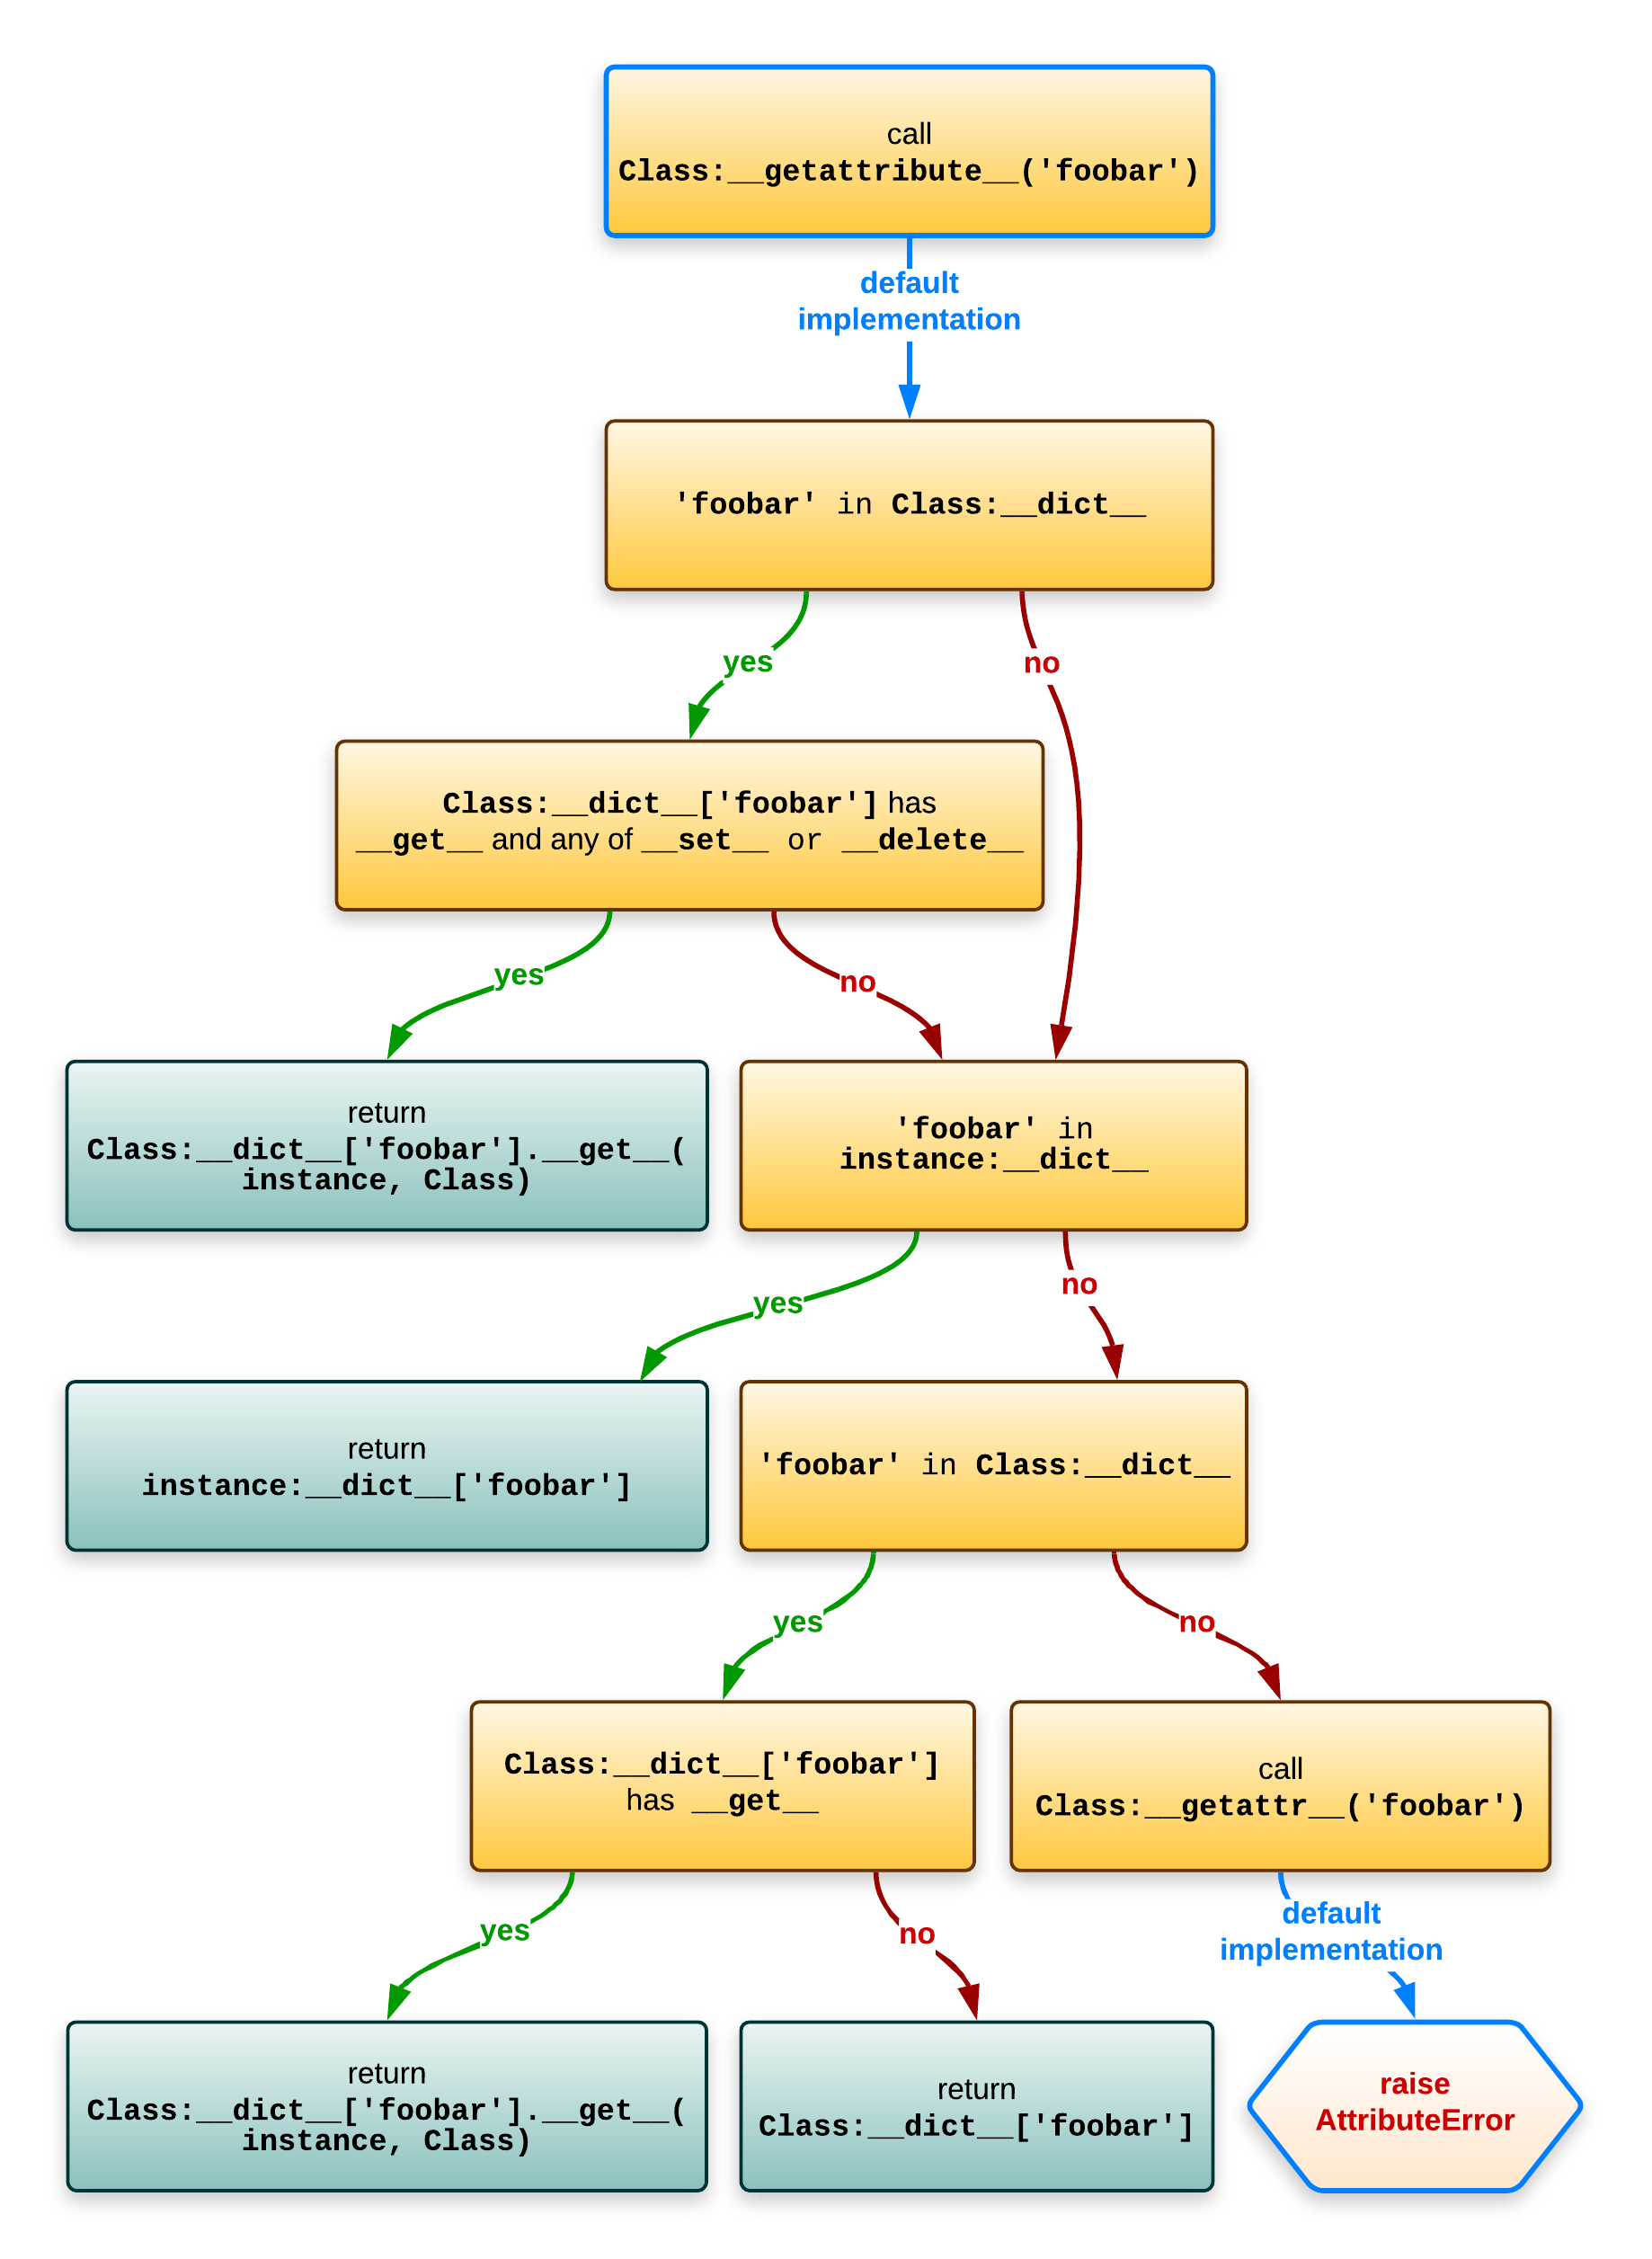
\includegraphics[width=.9\linewidth]{/Users/zhou/Documents/github/notes/python/object-attribute-lookup-v3.png}
\end{center}

\#+begin\textsubscript{src} python
\subsubsection{Assuming Class is the class and instance is an instance of Class, evaluating instance.foobar roughly equates to this:}
\label{sec:org101c358}
\subsubsection{(1).Call the type slot for Class.\_\textsubscript{getattribute}\_\_ (tp\textsubscript{getattro}). The default does this: [10]}
\label{sec:org9e824fe}
\subsubsection{(2).Does Class.\_\textsubscript{dict}\_\_ have a foobar item that has a \underline{\underline{get}} method and is a data descriptor [8]?}
\label{sec:org79bae76}
\subsubsection{(3).If yes, return the result of Class.\_\textsubscript{dict}\_\_['foobar'].\_\textsubscript{get}\_\textsubscript{(instance, Class)}. [6]}
\label{sec:orgbe5b179}
\subsubsection{(4).Does instance.\_\textsubscript{dict}\_\_ have a foobar item in it?}
\label{sec:orgeb03a2a}
\subsubsection{(5).If yes, return instance.\_\textsubscript{dict}\_\_['foobar'].}
\label{sec:orgb3b7f40}
\subsubsection{(6).Does Class.\_\textsubscript{dict}\_\_ have a foobar item that has a \underline{\underline{get}} method and is not a data descriptor [9]?}
\label{sec:org4b6a587}
\subsubsection{(7).If yes, return the result of Class.\_\textsubscript{dict}\_\_['foobar'].\_\textsubscript{get}\_\textsubscript{(instance, Class)}. [6]}
\label{sec:orgeeb66e8}
\subsubsection{(8).Does Class.\_\textsubscript{dict}\_\_ have a foobar item?}
\label{sec:org33fd87f}
\subsubsection{(9).If yes, return the result of Class.\_\textsubscript{dict}\_\_['foobar'].}
\label{sec:org9d2aead}
\subsubsection{(10).If the attribute still wasn't found, and there's a Class.\_\textsubscript{getattr}\_\_, call Class.\_\textsubscript{getattr}\_\textsubscript{('foobar')}.}
\label{sec:orgc299a00}
\subsection{Class attribute lookup:}
\label{sec:org2582e6a}
\begin{verbatim}
# Because classes needs to be able support the classmethod and staticmethod properties [6] when you evaluate some# thing like Class.
# foobar the lookup is slightly different than what would happen when you evaluate instance.foobar.
# Assuming Class is an instance of Metaclass, evaluating Class.foobar roughly equates to this:
# Call the type slot for Metaclass.__getattribute__ (tp_getattro). The default does this: [11]
# Does Metaclass.__dict__ have a foobar item that has a __get__ method and is a data descriptor [8]?
# If yes, return the result of Metaclass.__dict__['foobar'].__get__(Class, Metaclass). [6]
# Does Class.__dict__ have a foobar item that is a descriptor (of any kind)?
# If yes, return the result of Class.__dict__['foobar'].__get__(None, Class). [6]
# Does Class.__dict__ have a foobar item in it?
# If yes, return Class.__dict__['foobar'].
# Does Metaclass.__dict__ have a foobar item that is not a data descriptor [9]?
# If yes, return the result of Metaclass.__dict__['foobar'].__get__(Class, Metaclass). [6]
# Does Metaclass.__dict__ have any foobar item?
# If yes, return Metaclass.__dict__['foobar'].
# If the attribute still wasn't found, and there's a Metaclass.__getattr__, call Metaclass.__getattr__('foobar').
\end{verbatim}
\subsubsection{}
\label{sec:orgd9b5d29}
\#+end\textsubscript{src}
\section{实现底层@classmethod}
\label{sec:org54cf621}
\begin{verbatim}
class NewDefine_classmethod:
    """
    使用“描述符”和“装饰器”结合起来,模拟@classmethod
    """
    def __init__(self, function):
        self.function = function

    def __get__(self, instance, owner):
        #对传进函数进行加工,最后返回该函数
        def wrapper(*args, **kwargs):   #使用不定参数是为了匹配需要修饰的函数参数
            print("给函数添加额外功能")
            self.function(owner, *args, **kwargs)
        return wrapper

class Person:
    name='我有姓名'
    def __init__(self):
        pass
    @NewDefine_classmethod
    def study_1(cls):
        print(f'我的名字是:{cls.name},我会搞学习!')
    @NewDefine_classmethod
    def study_2(cls,score):
        print(f'我的名字是:{cls.name},我会搞学习!,而且这次考试考了 {score} 分')

print(Person.study_1())
print(Person.study_2(99))

# 第一步:@NewDefine_classmethod本质上是一个“类装饰器”,从它的定义可知,它的定义为
# class NewDefine_classmethod(function).我们发现,python系统定义的@classmethod其实它的定义也是一样的,如下,
# class classmethod(function) .怎么样?它们二者的定义是不是一样?
# 第二步:NewDefine_classmethod本质上又是一个描述符,因为在它的内部实现了__get__协议,由此可见,NewDefine_classmethod是“集装饰器-描述符”于一身的。
# 第三步:运行过程分析,因为study_1=NewDefine_classmethod(study_1),所以,study_1本质上是一个NewDefine_classmethod的对象,又因为NewDefine_classmethod本质上是实现了描述符的,所以,study_1本质上是一个定义在类中的描述符属性。
# 第四步:因为study_1本质上是一个定义在类中的描述符属性。所以在执行Person.study_1的时候,相当于是访问类的描述符属性,所以会进入到描述符的__get__方法。
# 注意:如果修饰的函数本身是具有返回值的,在__get__里面所定义的wrapper里面一定要返回,即return self.function(owner, *args, **kwargs)。
\end{verbatim}
\section{实现底层 @staticmethod}
\label{sec:org60b2b44}
\begin{verbatim}
class NewDefine_staticmethod:
    """
    使用“描述符”和“装饰器”结合起来,模拟@classmethod
    """
    def __init__(self, function):
        self.function = function

    def __get__(self, instance, owner):
        #对传进函数进行加工,最后返回该函数
        def wrapper(*args, **kwargs):   #使用不定参数是为了匹配需要修饰的函数参数
            print("给函数添加额外功能")
            self.function(*args, **kwargs)
        return wrapper

class Person:
    name='我有姓名'
    def __init__(self):
        pass

    @NewDefine_staticmethod
    def study_1(math,english):
        print(f'我数学考了 {math} 分,英语考了 {english} 分,我会搞学习!')

    @NewDefine_staticmethod
    def study_2(history,science):
        print(f'我历史考了 {history} 分,科学考了 {science} 分,我会搞学习!')

print(Person.study_1(99,98))
print(Person.study_2(88,89))
\end{verbatim}
\section{实现底层 @property}
\label{sec:org034431f}
\begin{verbatim}
class NewDefine_property:
    """
    使用“描述符”和“装饰器”结合起来,模拟@classmethod
    """
    def __init__(self, function):
        self.function = function

    def __get__(self, instance, owner):
        print("给函数添加额外功能")
        return self.function(instance)

class Person:
    name='我有姓名'
    def __init__(self):
        self.__study=100

    @NewDefine_property
    def study_1(self):  #使用property装饰的函数一般不要用“参数”,因为它的主要功能是对属性的封装
        return self.__study

p=Person()
print(p.study_1)
# 基本思想和前面分析的还是一样的,但是有几个地方有所区别,需要注意:
# 第一:@property的目的是封装一个方法,是这个方法可以被当做属性访问
# 第二:调用的方式与前面有所不同,__get__里面不能再定义wrapper了,否则不会调用wrapper。得不到想要的结果,为什么呢?
# 因为调用的方式不一样,根据前面的分析,study_1的本质是描述符属性,但是前面的调用均是使用的
# Person.study_1()或者是p.study_1()的形式,还是当成方法去使用的。但是此处不一样了,直接就是当成属性去使用,
# p.study_1 ,不再是方法调用,因此wrapper函数得不到调用。所以__get__方法得到了进一步简化。
\end{verbatim}
\section{描述器和装饰器的区别}
\label{sec:orge3a3574}
\subsection{同:描述器类和不带参数的装饰器类一样,都传入函数对象作为参数,并返回一个类实例}
\label{sec:org065fba2}
\subsection{异:装饰器类返回 callable 的实例,描述器则返回描述器实例}
\label{sec:org39ddf18}
\section{属性调用}
\label{sec:orgeb8bb72}
\subsection{整个描述符的核心是`\_\textsubscript{getattribute}\_\_`, 因为对每个属性实例的调用都会用到这个函数。这个方法被用来查找类属性,同时也是属性代理,调用该方法可以进行属性访问}
\label{sec:orgf283b64}
\subsubsection{给定类X和实例x, x.foo由`\_\textsubscript{getattribute}\_\_`转化为:type(x).\_\textsubscript{dict}['foo'].\_\textsubscript{get}\_\textsubscript{(x, type(x))},描述符是类属性,要用类调用}
\label{sec:orgb8336a9}
\begin{enumerate}
\item 对比定义:def `\_\textsubscript{get}\_\textsubscript{(self, instance, typ=None)}->value可知:self = type(x).\_\textsubscript{dict}\_\_['foo'], instance=x, typ=type(x)
\label{sec:org7316421}
\end{enumerate}
\subsubsection{如果是类调用了`\_\textsubscript{get}\_\_`方法,那么将None作为对象传入:X.\_\textsubscript{dict}['foo'].\_\textsubscript{get}\_\textsubscript{(None, X)}}
\label{sec:org2e0c771}
\begin{enumerate}
\item type.\_\textsubscript{getattribute}\_\textsubscript{()} 把 C.x 转化为 C.\_\textsubscript{dict}\_\_['x'].\_\textsubscript{get}\_\textsubscript{(None, C)}。
\label{sec:org5071c75}
\end{enumerate}
\subsubsection{非数据描述符的目的只是当实例属性值不存在时,提供一个值。当一个实例的`\_\textsubscript{dict}\_\_`中找不到某个属性时,才去调用`\_\textsubscript{getattr}\_\_`,如果没有找到非数据描述符,那么`\_\textsubscript{getattribute}\_\_`会抛出异常,然后调用`\_\textsubscript{getattr}\_\_`}
\label{sec:org1581afa}
\subsection{`\_\textsubscript{getattribute}\_\_`调用顺序}
\label{sec:org07429d1}
\subsubsection{类属性 > 数据描述符 > 实例属性(`\_\textsubscript{dict}\_\_['foo']`) > 非数据描述符 > `\_\textsubscript{getattr}\_\_`}
\label{sec:org4666bae}
\subsubsection{获取属性的三种方法:(a).instance.attr, (2).instance.\_\textsubscript{dict}\_\_['attr'], (3).getattr(instance, 'attr')}
\label{sec:orgab02e65}
\subsubsection{点操作符的查找逻辑位于 object.\_\textsubscript{getattribute}\_\textsubscript{()} 方法中}
\label{sec:org4edd554}
\subsubsection{一般情况下, 当调用instance.attr(点属性符)访问属性时,实际是使用instance.\_\textsubscript{dict}\_\_['attr']}
\label{sec:orgb90037f}
\subsubsection{`\_\textsubscript{setitem}\_\textsubscript{()}、`\_\textsubscript{getitem}\_\textsubscript{()}、`\_\textsubscript{delitem}\_\textsubscript{()}:`\_\textsubscript{xxxitem}\_\_:使用 [''] 的方式操作属性时被调用}
\label{sec:org45a5aeb}
\begin{enumerate}
\item `\_\textsubscript{setitem}\_\_:每当属性被赋值的时候都会调用该方法,因此不能再该方法内赋值 self.name = value 会死循环
\label{sec:orgab2f84d}
\item `\_\textsubscript{getitem}\_\_:当访问不存在的属性时会调用该方法
\label{sec:orgdd77491}
\item \underline{`\textsubscript{delitem}\_}:当删除属性时调用该方法
\label{sec:org010a2bf}
\end{enumerate}
\subsection{类的方法实际就是一个仅实现了 \_\textsubscript{get}\_\textsubscript{()} 的非资料描述器,所以如果实例 c 中同时定义了名为 foo 的方法和属性,那么 c.foo 访问的是属性而非方法。}
\label{sec:org617dd3a}

\begin{verbatim}
class Descriptor:
    def __init__(self, var1):
        print(f"descriptor init: {var1}")
        self.var1 = var1

    def __set__(self, instance, value):
        """"""
        print(f"Assigning {value}")

    def __get__(self, instance, owner=None):
        """"""
        print('Getting value')
        return "descriptor returned value"


class Person:

    foo = Descriptor("init")
    def __init__(self, value):
        self.foo = value

person = Person('instance') # descriptor init: init, Assigning instance
print("2", person.foo)      # Getting value, 2 descriptor returned value
person.foo ='test'          # Assigning test
print("3", person.foo)      # Getting value
# 给实例属性赋值时,由于数据描述符比实例属性优先级高,所以赋值被隐藏
\end{verbatim}
\subsection{有几点需要牢记的:}
\label{sec:org023ba1a}
\subsubsection{描述器被 \_\textsubscript{getattribute}\_\textsubscript{()} 方法调用,因而,重载 \_\textsubscript{getattribute}\_\textsubscript{()} 可能会妨碍描述器被自动调用}
\label{sec:orgce1df0f}
\subsubsection{\_\textsubscript{getattribute}\_\textsubscript{()} 仅存在于继承自 object 的新式类之中}
\label{sec:org9bd454e}
\subsubsection{object.\_\textsubscript{getattribute}\_\textsubscript{()} 和 type.\_\textsubscript{getattribute}\_\textsubscript{()} 对 \_\textsubscript{get}\_\textsubscript{()} 的调用不一样}
\label{sec:org22f2863}
\subsubsection{资料描述器总会覆盖实例字典,即资料描述器具有最高优先级}
\label{sec:org307d7c3}
\subsubsection{非资料描述器可能会被实例字典覆盖,即非资料描述器具有最低优先级}
\label{sec:org12c456b}

\subsection{property()是在它所在的类被创建时被调用的,所以传入property的参数是非绑定的函数(不是方法,因为实例没有创建)}
\label{sec:org24e0d17}

\section{yield from}
\label{sec:orge79e9cd}
\subsection{yield from 后面可以跟的可以是“ 生成器 、元组、 列表、range()函数产生的序列等可迭代对象”}
\label{sec:org4d289cd}
\subsection{yield from  generator, 实际上就是返回另外一个生成器. 而yield只是返回一个元素}
\label{sec:org33cab4a}
\subsection{yield from iterable本质上等于 for item in iterable: yield item}
\label{sec:orgfbef080}
\begin{verbatim}
def foo():
    print("starting...")
    while True:
        res = yield 4
        print("res:",res)
g = foo()
print(next(g))
print("*"*20)
print(next(g))

# starting...  
# 4      
# ********************
# res: None     下次调用generator从前面yield的下一句开始
# 4

# 1.程序开始执行以后,因为foo函数中有yield关键字,所以foo函数并不会真的执行,而是先得到一个生成器g(相当于一个对象)
# 2.直到调用next方法,foo函数正式开始执行,先执行foo函数中的print方法,然后进入while循环
# 3.程序遇到yield关键字,然后把yield想想成return,return了一个4之后,程序停止,并没有执行赋值给res操作,此时next(g)语句执行完成,所以输出的前两行(第一个是while上面的print的结果,第二个是return出的结果)是执行print(next(g))的结果,
# 4.程序执行print("*"*20),输出20个*
# 5.又开始执行下面的print(next(g)),这个时候和上面那个差不多,不过不同的是,这个时候是从刚才那个next程序停止的地方开始执行的,也就是要执行res的赋值操作,这时候要注意,这个时候赋值操作的右边是没有值的
#(因为刚才那个是return出去了,并没有给赋值操作的左边传参数),所以这个时候res赋值是None,所以接着下面的输出就是res:None,
# 6.程序会继续在while里执行,又一次碰到yield,这个时候同样return 出4,然后程序停止,print函数输出的4就是这次return出的4.

# 到这里你可能就明白yield和return的关系和区别了,带yield的函数是一个生成器,而不是一个函数了,这个生成器有一个函数就是next函数,next就相当于“下一步”生成哪个数,这一次的next开始的地方是接着上一次的next停止的地方执行的,所以调用next的时候,
# 生成器并不会从foo函数的开始执行,只是接着上一步停止的地方开始,然后遇到yield后,return出要生成的数,此步就结束。

\end{verbatim}

\begin{verbatim}
def foo():
    print("starting...")
    while True:
        res = yield 4 # 下一句是赋值
        print("res:",res)
g = foo()
print(next(g))
print("*"*20)
print(g.send(7)) 

# starting...
# 4
# ********************
# res: 7
# 4

# send是发送一个参数给res的,因为上面讲到,return的时候,并没有把4赋值给res,下次执行的时候只好继续执行赋值操作,只好赋值为None了,而如果用send的话,开始执行的时候,
# 先接着上一次(return 4之后)执行,先把7赋值给了res,然后执行next的作用,遇见下一回的yield,return出结果后结束。

\end{verbatim}
\subsection{yield from 替代内层for循环}
\label{sec:orge526916}
\subsubsection{如果生成器函数需要产出另一个生成器生成的值,传统的解决方法是使用嵌套的for循环}
\label{sec:org74b0a4d}
\begin{verbatim}
def chain(*iterables):
    for it in iterables:
        for i in it:
            yield i

s = 'ABC'
t = tuple(range(3))
# chain 生成器函数把操作依次交给接收到的各个可迭代对象处理。
list(chain(s, t))
\end{verbatim}
\begin{verbatim}
def chain(*iterables):
    for i in iterables:
        yield from i
list(chain(s, t))

# yield from 完全代替了内层的 for 循环。
# yield from x 表达式对 x 对象所做的第一件事是,调用 iter(x),从中获取迭代器。因此,x 可以是任何可迭代的对象。

\end{verbatim}

\begin{verbatim}
# 我们有一个嵌套型的序列,想将它扁平化处理为一列单独的值
from collections import Iterable

def flatten(items, ignore_types=(str, bytes)):
    for x in items:
        if isinstance(x, Iterable) and not isinstance(x, ignore_types):
            yield from flatten(x)
        else:
            yield x

items = [1, 2, [3, 4, [5, 6], 7], 8]
for x in flatten(items):
    print(x)
# collections.Iterable是一个抽象基类,我们用isinstance(x, Iterable)检查某个元素是否是可迭代的.如果是的话,那么就用yield from将这个可迭代对象作为一种子例程进行递归。最终返回结果就是一个没有嵌套的单值序列了。    
\end{verbatim}

\begin{verbatim}
# 利用一个Node类来表示树结构
class Node:
    def __init__(self, value):
        self._value = value
        self._children = []

    def __repr__(self):
        return 'Node({!r})'.format(self._value)

    def add_child(self, node):
        self._children.append(node)

    def __iter__(self):
        return iter(self._children)

    def depth_first(self):
        yield self
        for c in self:
            yield from c.depth_first()

if __name__ == '__main__':
    root = Node(0)
    child1 = Node(1)
    child2 = Node(2)
    root.add_child(child1)
    root.add_child(child2)
    child1.add_child(Node(3))
    child1.add_child(Node(4))
    child2.add_child(Node(5))
    for ch in root.depth_first():
        print(ch)

# __iter__代表一个Pyton的迭代协议,返回一个迭代器对象,就能迭代了
# depth_frist返回一个生成器,仔细体会其中的yield与 yield from用法        
\end{verbatim}


\begin{verbatim}
# 我们都知道,在使用yield生成器的时候,如果使用for语句去迭代生成器,则不会显式的出发StopIteration异常,而是自动捕获
# StopIteration异常,所以如果遇到return,只是会终止迭代,而不会触发异常,故而也就没办法获取return的值。
def my_generator():
    for i in range(5):
        if i==2:
            return '我被迫中断了'
        else:
            yield i

def main(generator):
    try:
        # 迭代到2的时候遇到return语句,隐式的触发了StopIteration异常,就终止迭代了,但是在程序中不会显示出来。
        for i in generator:  #不会显式触发异常,故而无法获取到return的值
            print(i)
    except StopIteration as exc:
        print(exc.value)

g=my_generator()  #调用
\end{verbatim}
\begin{verbatim}
def my_generator():
    for i in range(5):
        if i==2:
            return '我被迫中断了'
        else:
            yield i

def wrap_my_generator(generator):  #定义一个包装“生成器”的生成器,它的本质还是生成器
    result=yield from generator    #自动触发StopIteration异常,并且将return的返回值赋值给yield from表达式的结果,即result
    print(result)

def main(generator):
    for j in generator:
        print(j)

g=my_generator()
wrap_g=wrap_my_generator(g)
# 从上面的比较可以看出,yield from具有以下几个特点:
# (1)上面的my_generator是原始的生成器,main是调用方,使用yield的时候,只涉及到这两个函数,即“调用方”与“生成器(协程函数)”是直接进行交互的,不涉及其他方法,即“调用方——>生成器函数(协程函数)”;
# (2)在使用yield from的时候,多了一个对原始my_generator的包装函数,然后调用方是通过这个包装函数(后面会讲到它专有的名词)来与生成器进行交互的,即“调用方——>生成器包装函数——>生成器函数(协程函数)”;
# (3)yield from iteration结构会在内部自动捕获 iteration生成器的StopIteration 异常。这种处理方式与 for 循环处理 StopIteration 异常的方式一样。而且对 yield from 结构来说,
# 解释器不仅会捕获 StopIteration 异常,还会把return返回的值或者是StopIteration的value 属性的值变成 yield from 表达式的值,即上面的result。
\end{verbatim}

\section{magic method}
\label{sec:orgcdce184}

\begin{verbatim}
# __missing__(self, i): what to do when dict key i is missing
# __contains__(self, i): Behaviour for in and not in operators, value in self, value not in self
# __iter__(self): returns the iterator object itself, obj with __iter__ is iterable
# __next__(self): either return the next item or must raise StopIteration. Notes, iterator has both __iter__ and __next__ methods
# __index__(self): Called by x[self], 当对象是被应用在切片表达式中时,实现整形强制转换, return an int
# __setattr__(self, name, val): called by self.name = val
# __getattribute__(self, name):  Called by self.name
# __getattr__(self, name): called when self.name does not exist
# __delattr__(self, name):  Called by del self.name
# __getitem__(self,key): Called by self[key], it is important to slicing
# __setitem__(self, key, val): Called by self[key] = val
# __delitem__(self, key): called by del self.key
# __concat__(self, value):	self + other	连接两个对象时
# __call__(self [,...]):	self(args)	“调用”对象时
# __enter__(self):	with self as x:	with 语句环境管理
# __exit__(self, exc, val, trace):	with self as x:	with 语句环境管理

# Note:
# 1. An object can be iterated over with "for" if it implements __iter__() or __getitem__().
# 2. An object can function as an iterator if it implements next().
\end{verbatim}

\section{exceptional flow control}
\label{sec:org1ed4688}
\begin{verbatim}
try:
    statements
except (tuple_of_errors): # can have multiple
    statements
else: # optional no exceptions
    statements
finally: # optional all circumstances
    statements
\end{verbatim}

\begin{verbatim}
# common exceptions
# AsserionError: Assert statement failed
# AttributeError: Class attribute assignment or reference failed
# IOErro: Failed I/O operation Failed module import Subscript out of range Dictionary key not found Ran out of memory
# ImportError: Failed module import
# IndexError: Subscript out of range
# KeyError: Dictionary key not found
# MemoryError: Ran out of memory
# NameError: Name not found
# TypeError: Value of the wrong type
# ValueError: Right type but wrong value
\end{verbatim}

\section{July 13, 2021}
\label{sec:orgec576e5}
\subsection{jupyter-lab cannot find my env}
\label{sec:org89dc20f}

\subsection{solutions}
\label{sec:org000434f}
\begin{itemize}
\item Assuming your conda-env is named cenv, it is as simple as :
\item conda activate cenv
\item (cenv)\$ conda install ipykernel
\item (cenv)\$ ipython kernel install --user --name=<any\textsubscript{name}\textsubscript{for}\textsubscript{kernel}>
\item (cenv(\$ conda deactivate
\item If you restart your jupyter notebook/lab you will be able to see the new kernel available.
\item PS: If you are using virtualenv etc. the above steps hold good.
\end{itemize}

links: \url{https://jupyter.org/install}


\subsection{Machine learning course links}
\label{sec:org08cda45}
\subsubsection{{\bfseries\sffamily TODO} \url{https://speech.ee.ntu.edu.tw/\~hylee/mlds/2018-spring.html}}
\label{sec:org36c1b1e}
\subsubsection{{\bfseries\sffamily TODO} statistics review: \url{https://zhuanlan.zhihu.com/p/70034585}}
\label{sec:org4296d83}
\subsubsection{python tutorials}
\label{sec:orgeec2711}
\begin{enumerate}
\item {\bfseries\sffamily TODO} \url{https://blog.csdn.net/liuchunming033/category\_1348374.html}
\label{sec:org5e2d6ec}
\item {\bfseries\sffamily TODO} vis training and loss: \url{https://machinelearningmastery.com/learning-curves-for-diagnosing-machine-learning-model-performance/}, \url{https://blog.csdn.net/bbbeoy/article/details/113503988}, \url{https://oldpan.me/archives/how-to-use-tricks-to-train-network}
\label{sec:orgc7a78b6}
\end{enumerate}
\subsubsection{pytorch tutorials:}
\label{sec:org823b195}
\begin{enumerate}
\item \url{https://blog.csdn.net/u012436149/category\_9268433.html?spm=1001.2014.3001.5482}
\label{sec:org5619392}
\item \url{https://blog.csdn.net/qq\_27825451/article/details/96837905}
\label{sec:org28fad2a}
\item \url{https://pytorch.org/tutorials/beginner/basics/quickstart\_tutorial.html}
\label{sec:org7d6ccdc}
\end{enumerate}
\subsubsection{Design patterns tutorials:}
\label{sec:orgcf6ef17}
\begin{enumerate}
\item \url{https://python-web-guide.readthedocs.io/zh/latest/design/design.html\#the-fctory-pattern}
\label{sec:orgc61368c}
\item \url{https://refactoringguru.cn/design-patterns/abstract-factory}
\label{sec:org0968094}
\end{enumerate}
\subsubsection{tensorflow tutorials}
\label{sec:org5b973ad}
\begin{enumerate}
\item \url{https://blog.csdn.net/u012436149/category\_9267152\_2.html}
\label{sec:org245b02d}
\end{enumerate}
\subsubsection{XAI vis}
\label{sec:org7a41421}
\begin{enumerate}
\item \url{https://github.com/interpretml/interpret}
\label{sec:orgc6b7748}
\end{enumerate}
\section{python attribute lookup order}
\label{sec:org33136f8}
\subsection{\url{https://blog.ionelmc.ro/2015/02/09/understanding-python-metaclasses/\#object-attribute-lookup}}
\label{sec:orgb77c95a}
\subsection{}
\label{sec:org89a499d}
\end{document}